\documentclass[11pt]{article}
\usepackage[a4paper,margin=1in]{geometry}
\usepackage{lmodern}
\usepackage[T1]{fontenc}
\usepackage{microtype}
\usepackage{amsmath,amssymb,amsthm,bm}
\usepackage{mathtools}
\usepackage{booktabs}
\usepackage{enumitem}
\usepackage{hyperref}
\usepackage{cleveref}
\usepackage{algorithm}
\usepackage{algpseudocode}
\usepackage{tikz}
\usetikzlibrary{arrows.meta,positioning,calc,fit,shapes.misc,shapes.geometric, calc, bayesnet}
% \usetikzlibrary{bayesnet, arrows, positioning, fit, shapes.geometric}
\newcommand{\vecs}[1]{\boldsymbol{#1}} % For vectors, e.g., alpha, mu
\theoremstyle{definition}
\newtheorem{definition}{Definition}
\newtheorem{proposition}{Proposition}
\newtheorem{remark}{Remark}
\newtheorem{lemma}{Lemma}
\newcommand{\Feedback}{\mathsf{Feedback}}
\title{Learning to Defer For Time Series via Switching State-Space Models}
\author{}
\date{\today}

\newcommand{\E}{\mathbb{E}}
\newcommand{\Var}{\mathrm{Var}}
\newcommand{\Cov}{\mathrm{Cov}}
\newcommand{\1}{\mathbf{1}}
\newcommand{\R}{\mathbb{R}}
\newcommand{\given}{\,\middle|\,}
\newcommand{\Normal}{\mathcal{N}}
\newcommand{\N}{\mathbb{N}}
\newcommand{\I}{\mathcal{I}}  % Information set
\newcommand{\Regime}{\mathcal{Z}} % Regime space
\newcommand{\Expert}{\mathcal{K}} % Expert set
\newcommand{\trans}{^{\top}}


\newcommand{\bmalpha}{\vecs{\alpha}}
\newcommand{\bmSigma}{\vecs{\Sigma}}
\newcommand{\bmK}{\vecs{K}}

\begin{document}
\maketitle




\begin{abstract}
We present a theoretical framework for Learning-to-Defer (L2D) in non-stationary time series environments where querying experts incurs an explicit consultation cost. We formalize the problem as a sequential decision process under partial observation with a time-varying set of experts. We model the time-varying reliability of black-box experts (e.g., neural networks) as latent states in a Switching Linear Dynamical System (SLDS). This structure captures abrupt environmental shifts (regimes) and gradual performance drift. We derive a tractable inference algorithm using the Interacting Multiple Model (IMM) filter, providing full derivations for the variance spread in Gaussian mixtures, and propose a cost-sensitive myopic selection policy that balances predictive risk, epistemic uncertainty, and operational costs.
\end{abstract}

Note: might be interested to predict when the expert will be or not available?

\section{Problem Formulation}

\subsection{Preliminaries}

We consider a sequential forecasting and routing problem over a discrete horizon
$t=1,\dots,T$. All random quantities are defined on a probability space
$(\Omega,\mathcal{F},\mathbb{P})$ equipped with a filtration
$\mathbb{F}=\{\mathcal{F}_t\}_{t\ge1}$.
Throughout, we interpret $\mathcal{F}_t$ as the information available to the router
\emph{at decision time} $t$, i.e.\ immediately \emph{before} selecting an expert at time $t$.

\begin{itemize}
    \item \textbf{Context and Target (Regression Setting).}
    At each time $t$, nature reveals a context vector $\mathbf{x}_t \in \mathcal{X}\subseteq\mathbb{R}^d$.
    The router observes $\mathbf{x}_t$ at decision time, so $\mathbf{x}_t$ is $\mathcal{F}_t$-measurable.
    The associated ground-truth target is
    \[
        y_t \in \mathcal{Y}\subseteq\mathbb{R},
    \]
    which is \emph{not} observed at decision time; in particular, $y_t$ need not be $\mathcal{F}_t$-measurable.

    \item \textbf{Dynamic Expert Registry (The Roster).}
    We distinguish between the set of experts currently available and the set of experts known to the system.
    Let $\mathcal{U}_t$ denote the \emph{registry} of all experts encountered up to time $t$.
    This registry evolves cumulatively to preserve the learned history of temporarily unavailable experts:
    \[
        \mathcal{U}_t \coloneqq \mathcal{U}_{t-1} \cup \Expert_t \qquad (\text{with } \mathcal{U}_0 = \varnothing).
    \]

    \item \textbf{Expert Availability.}
    At decision time $t$, only a subset $\Expert_t \subseteq \mathcal{U}_t$ is available for querying.
    We assume $\Expert_t$ is observed at decision time (hence $\mathcal{F}_t$-measurable) and
    \[
        \mathbb{P}(\Expert_t \neq \varnothing)=1 \qquad \text{for all } t=1,\dots,T.
    \]

    \item \textbf{Expert predictions.}
    Each expert $j\in\mathcal{U}_t$ is associated with a prediction rule
    $f_j:\mathcal{X}\to\mathcal{Y}$ (deterministic, or more generally $\mathcal{F}_1$-measurable and fixed over time).
    If $j\in\Expert_t$, then at time $t$ expert $j$ returns
    \[
        \hat{y}_t^{(j)} \coloneqq f_j(\mathbf{x}_t).
    \]

    \item \textbf{Latent regimes and expert dependence (standing modeling scope).}
    Our generative model (introduced later) includes a latent regime process $(z_t)_{t\ge1}$ whose transitions may depend on
    the observed contexts (context-dependent switching), and a shared latent factor $(g_t)_{t\ge1}$ that can induce
    \emph{correlations across experts} at a fixed time $t$.
    In particular, we do \emph{not} assume that the losses $(\ell_{j,t})_{j\in\mathcal{U}_t}$ are independent across $j$.

    \item \textbf{Loss process and bandit (censored) feedback.}
    Performance is evaluated through a loss function
    \[
        \mathcal{L}:\mathcal{Y}\times\mathcal{Y}\to[0,+\infty).
    \]
    The (counterfactual) instantaneous loss of expert $j$ at time $t$ is the random variable
    \[
        \ell_{j,t} \coloneqq \mathcal{L}\!\bigl(\hat{y}_t^{(j)},y_t\bigr)\in[0,+\infty).
    \]
    We assume $\{\ell_{j,t}:j\in\mathcal{U}_t,\,t=1,\dots,T\}$ is a well-defined collection of random variables
    on $(\Omega,\mathcal{F},\mathbb{P})$, potentially dependent across experts at a given time $t$.
    Under bandit (censored) feedback, once the router selects an expert index $r_t\in\Expert_t$ at time $t$,
    it observes only the realized loss $\ell_{r_t,t}$, while $\{\ell_{j,t}:j\neq r_t\}$ remain unobserved.
    Concretely, $\ell_{r_t,t}$ is not assumed to be $\mathcal{F}_t$-measurable, but is revealed after the decision at time $t$
    and hence becomes measurable with respect to $\mathcal{F}_{t+1}$.

    \item \textbf{History and admissible policies.}
    Define the end-of-round feedback random element
    \[
        F_t \coloneqq (r_t,\ell_{r_t,t}) \in \mathcal{U}_t\times[0,+\infty).
    \]
    The interaction history available at decision time $t$ (i.e., up to round $t-1$) is
    \[
        \mathcal{I}_{t-1} \coloneqq \bigl((\mathbf{x}_\tau,\Expert_\tau,F_\tau)\bigr)_{1\le \tau \le t-1},
        \qquad \mathcal{I}_0 \text{ empty}.
    \]
    The information available at decision time $t$ is summarized by
    \[
        H_t \coloneqq (\mathcal{I}_{t-1},\mathbf{x}_t,\Expert_t).
    \]
    We take the observation filtration to be generated by this information:
    \[
        \mathcal{F}_t = \sigma(H_t), \qquad t=1,\dots,T.
    \]
    A (deterministic) routing policy is a sequence of measurable maps
    \[
        \pi_t:\mathsf{H}_t\to\mathcal{U}_t, \qquad t=1,\dots,T,
    \]
    where $\mathsf{H}_t$ denotes the measurable space in which $H_t$ takes values, and such that
    $\pi_t(H_t)\in\Expert_t$ almost surely.
    The chosen expert at time $t$ is
    \[
        r_t \coloneqq \pi_t(H_t),
    \]
    and in particular $r_t$ is $\mathcal{F}_t$-measurable with values in $\Expert_t$ almost surely.
\end{itemize}

\paragraph{Running Example (Medical Triage).}
Consider an automated triage system in a hospital Emergency Room.
\begin{itemize}
    \item The \textbf{Context} $\mathbf{x}_t$ represents a patient's initial vitals, laboratory values, and presenting symptoms.
    \item The \textbf{Target} $y_t$ is a real-valued outcome, e.g., a risk score or a biomarker observed after further testing.
    \item The \textbf{Experts} in $\Expert_t$ are diagnostic models or human specialists currently available (e.g., an on-call cardiologist).
          The set $\Expert_t$ varies over time. The system maintains a \textbf{Registry} $\mathcal{U}_t$ to track the reliability of all specialists, even those currently off-duty, allowing for immediate calibrated use upon their return.
    \item The \textbf{Loss} $\ell_{j,t}$ quantifies discrepancy between $f_j(\mathbf{x}_t)$ and $y_t$ (e.g., squared error).
          Only $\ell_{r_t,t}$ for the selected expert $r_t$ is observed and enters future decisions.
    \item \textbf{Non-stationarity} can arise both from distribution shifts that change expert performance over time
          and from regime switches whose transition behavior depends on the observed context.
\end{itemize}
The router must therefore select at each time $t$ an expert $r_t\in\Expert_t$ using only $(\mathbf{x}_t,\Expert_t)$ and the past history $\mathcal{I}_{t-1}$,
without observing $y_t$ (or the full loss vector $(\ell_{j,t})_{j\in\mathcal{U}_t}$) at decision time.

\subsection{The Decision Process}

The system operates as a \emph{cost-sensitive router}.
At each decision epoch $t\in\{1,\dots,T\}$, after observing
\[
    H_t = (\mathcal I_{t-1},\mathbf x_t,\Expert_t),
\]
the router selects a single expert index $r_t\in \Expert_t$ to query.

\begin{itemize}
    \item \textbf{Action space.}
    The admissible actions at time $t$ are exactly the currently available experts,
    i.e.\ the finite set $\Expert_t$. Note that $\Expert_t \subseteq \mathcal{U}_t$ (the current registry).
    The router chooses
    \[
        r_t \in \Expert_t.
    \]

    \item \textbf{Consultation costs.}
    Each expert $j\in\mathcal{U}_t$ is associated with a deterministic, nonnegative consultation cost
    \[
        \beta_j \ge 0,
    \]
    modeling, e.g., API fees, latency, computational/energy cost, or operational constraints.
    The cost vector $(\beta_j)_{j\in\mathcal{U}_t}$ is assumed known for all registered experts (persisting in memory even when experts are temporarily unavailable/offline).
\end{itemize}

\paragraph{Realized cost.}
Given an action $r_t\in\Expert_t$, the \emph{total realized cost} at time $t$ is
\begin{equation}\label{eq:realized_cost}
    C_t(r_t)
    \;\coloneqq\;
    \underbrace{\ell_{r_t,t}}_{\text{prediction loss}}
    \;+\;
    \underbrace{\beta_{r_t}}_{\text{consultation cost}}.
\end{equation}
At decision time $t$, $\beta_{r_t}$ is known, whereas $\ell_{r_t,t}$ is random.
Under bandit feedback, $\ell_{r_t,t}$ is revealed only after taking the action, and is incorporated into the next
decision via the updated history $\mathcal I_t$ (hence it is $\mathcal F_{t+1}$-measurable).

\paragraph{Objective.}
A (deterministic, possibly non-stationary) policy is a measurable sequence
$\pi=(\pi_t)_{t=1}^T$ such that $\pi_t(H_t)\in\Expert_t$ almost surely; the action is
$r_t \coloneqq \pi_t(H_t)$.
The goal is to minimize the expected cumulative cost over the horizon:
\begin{equation}
    \label{eq:objective}
    \inf_{\pi}
    \;
    \mathbb{E}
    \left[
        \sum_{t=1}^T C_t\bigl(\pi_t(H_t)\bigr)
    \right]
    \;=\;
    \inf_{\pi}
    \;
    \mathbb{E}
    \left[
        \sum_{t=1}^T
        \Bigl(
            \ell_{\pi_t(H_t),t}
            + \beta_{\pi_t(H_t)}
        \Bigr)
    \right].
\end{equation}
We call any policy $\pi^\star$ achieving the infimum (if it exists) \emph{optimal}. More generally, for $\varepsilon>0$,
a policy $\pi$ is \emph{$\varepsilon$-optimal} if its objective value is within $\varepsilon$ of the infimum in
\eqref{eq:objective}.

\paragraph{POMDP formulation (latent state and information state).}
To make explicit the control structure induced by censored feedback, we posit an unobserved latent state process
$(S_t)_{t=1}^T$ taking values in a measurable space $\mathcal S$ (which naturally expands as the registry grows) such that:

\begin{enumerate}[label=(\roman*)]
    \item \textbf{Emission model.} For each $t$ and each expert $j\in\mathcal{U}_t$ (the current registry), the loss $\ell_{j,t}$ admits a
    regular conditional distribution given $(S_t,\mathbf x_t)$ (hence also for the observed loss $\ell_{r_t,t}$),
    and the one-step cost is $C_t(j)=\ell_{j,t}+\beta_j$.

    \item \textbf{Context-dependent latent dynamics.} There exists a (possibly time-inhomogeneous) Markov kernel
    $\mathsf T_t(\cdot \mid s,\mathbf x_{t+1})$ such that, for all measurable $A\subseteq\mathcal S$,
    \[
        \mathbb P(S_{t+1}\in A \mid S_{1:t},\mathbf x_{1:t+1}, r_{1:t})
        \;=\;
        \mathsf T_t(A \mid S_t,\mathbf x_{t+1}).
    \]
    (In particular, the latent dynamics do not depend on the router's actions beyond what is already encoded in $S_t$ and the exogenous input $\mathbf x_{t+1}$.)

    \item \textbf{Encoding non-stationarity and cross-expert dependence (Option A).}
    The state $S_t$ is rich enough to encode (a) non-stationarity, e.g.\ through a regime component $z_t$, and
    (b) cross-expert dependence through shared latent factors, so experts need not be conditionally independent
    given the regime. The dimensionality of $S_t$ adapts to include latent variables for all experts in $\mathcal{U}_t$.
\end{enumerate}

The router does not observe $S_t$ directly; instead it observes $H_t$ at decision time and the end-of-round feedback
\[
    F_t=(r_t,\ell_{r_t,t})
\]
after acting. The \emph{belief state} at decision time $t$ is the posterior distribution
\[
    b_t(\cdot) \;\coloneqq\; \mathbb{P}\!\left(S_t \in \cdot \mid H_t\right).
\]
To make the control problem Markov, we use the \emph{information state}
\[
    I_t \;\coloneqq\; (b_t,\mathbf x_t,\Expert_t).
\]
Under the above assumptions (and standard measurability conditions), there exists a measurable filtering update map
$\tau_t$ such that, almost surely,
\[
    b_{t+1}
    \;=\;
    \tau_t\!\bigl(b_t,\mathbf x_t,\Expert_t, F_t, \mathbf x_{t+1},\Expert_{t+1}\bigr).
\]

\begin{proposition}[Information-state optimality and Bellman recursion]\label{prop:belief_pomdp}
Assume that $(S_t)$ evolves according to the context-dependent Markov kernel $\mathsf T_t$ above, and that the belief update
$b_{t+1}=\tau_t(\cdot)$ is well-defined and measurable. Assume also that $C_t(j)$ is integrable for all $t$ and $j$.
Then there exists an optimal policy for \eqref{eq:objective} that is Markov in the information state, i.e.\ of the form
\[
    r_t = \mu_t(b_t,\mathbf x_t,\Expert_t)
\]
for measurable decision rules $\mu_t$.
Moreover, defining $V_{T+1}\equiv 0$ and, for $t=T,\dots,1$,
\[
    V_t(b,\mathbf x,\Expert)
    \;\coloneqq\;
    \inf_{j\in\Expert}
    \Bigl\{
        \underbrace{\mathbb E\!\left[C_t(j)\mid b,\mathbf x\right]}_{\text{one-step Bayes risk}}
        \;+\;
        \mathbb E\!\left[V_{t+1}(b_{t+1},\mathbf x_{t+1},\Expert_{t+1})
        \mid b,\mathbf x,\Expert, j\right]
    \Bigr\},
\]
an optimal policy can be obtained by selecting at each time $t$ any minimizer of the right-hand side.
\end{proposition}


\paragraph{Intuition (The ``Economy of Diagnosis'').}
In the medical triage example, consider two experts:
\begin{itemize}
    \item \textbf{Expert A (Nurse Algorithm):} modest accuracy on complex cases, but very cheap (e.g., $\beta_A \approx 0$);
    \item \textbf{Expert B (Specialist):} high accuracy, but expensive or slow (e.g., $\beta_B \gg 0$).
\end{itemize}
A purely accuracy-driven scheme (ignoring $\beta_j$) might always select Expert~B whenever it yields smaller expected loss.
The cost-sensitive objective \eqref{eq:objective} forces a trade-off:
\emph{is the expected reduction in prediction loss from consulting the specialist worth the additional cost $\beta_B$?}
For contexts $\mathbf x_t$ indicating low risk, the router may select the cheaper model; for ambiguous or high-risk cases,
it may pay $\beta_B$ and consult the specialist.

\begin{remark}[Bayes action under squared loss]\label{rem:bayes_action_squared}
Assume that at time $t$ the router knows (or models) the conditional distribution of $y_t$ given $H_t$, and that the
instantaneous cost of choosing expert $j\in\Expert_t$ is
\[
    C_t(j) \coloneqq \bigl(f_j(\mathbf x_t) - y_t\bigr)^2 + \beta_j.
\]
Let $m_t \coloneqq \mathbb E[y_t \mid H_t]$ denote the conditional mean. Then a Bayes action at time $t$ is any minimizer
\[
    j_t^\star \in \arg\min_{j\in\Expert_t}
    \left\{
        \bigl(f_j(\mathbf x_t) - m_t\bigr)^2 + \beta_j
    \right\}.
\]
\end{remark}

\section{Generative Model: Switching Linear Dynamical System}

To construct a cost-sensitive routing policy, we require (or approximate), at each decision time $t$,
the conditional predictive law of each available expert's loss,
\[
    \mathbb{P}\bigl(\ell_{j,t}\mid H_t\bigr), \qquad j\in\Expert_t,
\]
where $H_t=(\mathcal I_{t-1},\mathbf x_t,\Expert_t)$ is the decision-time information defined in
Section~\ref{sec:preliminaries}. A static regression model $\ell_{j,t}=g_j(\mathbf x_t)+\varepsilon_{j,t}$ is
inadequate because (i) expert performance is non-stationary (drift and abrupt shifts), and (ii) under bandit
feedback we only observe $\ell_{r_t,t}$ for the selected expert $r_t$, so the loss process is partially observed.

We therefore posit that the counterfactual loss vector $(\ell_{j,t})_{j\in\mathcal{U}_t}$ is generated by an
\emph{input-driven Switching Linear Dynamical System} (SLDS): a discrete regime process controls the parameters of
continuous latent states that encode expert reliability, and these latent states are allowed to be \emph{correlated
across experts} through shared latent factors (Option~A).

\paragraph{Exogeneity.}
We adopt an exogeneity assumption: the latent environment
\[
    \bigl(z_t,\, g_t,\, (\mathbf u_{j,t})_{j\in\mathcal{U}_t}\bigr)_{t\ge1}
\]
evolves independently of the chosen indices $(r_t)_{t\ge1}$ (and, in particular, the router only affects which
component $\ell_{r_t,t}$ is revealed). The availability sets $(\Expert_t)$ and contexts $(\mathbf x_t)$ are treated
as observed exogenous inputs.

\subsection{Latent State Dynamics}

The SLDS combines (i) a discrete regime $z_t$ and (ii) regime-dependent linear-Gaussian dynamics for continuous latent
states. To encode cross-expert dependence parsimoniously, we use a shared-factor decomposition.

\paragraph{1. Regime process (discrete, context-dependent).}
Let
\[
    z_t \in \mathcal Z \coloneqq \{1,\dots,M\}
\]
be a discrete latent variable representing the global environmental regime at time $t$
(e.g., \emph{normal operations} vs.\ \emph{outbreak}). We allow the regime transitions to depend on the (exogenous)
context via an input-driven Markov chain: for $t\ge2$,
\begin{equation}
    \label{eq:regime_transition}
    \mathbb{P}\!\left(z_t=k \mid z_{t-1}=i,\,\mathbf x_t\right)= \Pi_{ik}(\mathbf x_t),
    \qquad
    \sum_{k=1}^M  \Pi_{ik}(\mathbf x)=1 \;\;\; \forall\, i,\ \forall\,\mathbf x\in\mathcal X,
\end{equation}
with an initial law that may also depend on $\mathbf x_1$, e.g.
\[
    \mathbb P(z_1=k\mid \mathbf x_1)=\mu_k^0(\mathbf x_1),\qquad k=1,\dots,M.
\]
The time-homogeneous Markov chain is recovered as the special case $ \Pi_{ik}(\mathbf x)\equiv  \Pi_{ik}$ and
$\mu^0(\mathbf x_1)\equiv \mu^0$.

\paragraph{2. Reliability state with shared latent factors (continuous).}
Fix a dimension $d_\alpha$. For each expert $j\in\mathcal{U}_t$ (the current registry), we define a latent reliability state
$\bm\alpha_{j,t}\in\mathbb R^{d_\alpha}$ through the decomposition
\begin{equation}
    \label{eq:factor_decomp}
    \bm\alpha_{j,t}
    \;\coloneqq\;
    B_j\, g_t + \mathbf u_{j,t},
\end{equation}
where
$g_t\in\mathbb R^{d_g}$ is a \emph{global} continuous factor shared by all experts, $B_j\in\mathbb R^{d_\alpha\times d_g}$
is an expert-specific loading matrix, and $\mathbf u_{j,t}\in\mathbb R^{d_\alpha}$ is an expert-specific idiosyncratic
state. This construction induces cross-expert dependence through the shared factor $g_t$ even when the idiosyncratic
components $(\mathbf u_{j,t})_j$ are conditionally independent.

\paragraph{3. Linear-Gaussian dynamics (regime-dependent).}
Conditional on the regime $z_t=k$, we posit linear-Gaussian transitions
\begin{align}
    \label{eq:global_factor_transition}
    g_t
    &= A_k^{(g)}\, g_{t-1} + \mathbf w_t^{(g)},
    &\mathbf w_t^{(g)} &\sim \mathcal N(\mathbf 0, Q_k^{(g)}),
    \\
    \label{eq:idiosyncratic_transition}
    \mathbf u_{j,t}
    &= A_k^{(u)}\, \mathbf u_{j,t-1} + \mathbf w_{j,t}^{(u)},
    &\mathbf w_{j,t}^{(u)} &\sim \mathcal N(\mathbf 0, Q_{k}^{(u)}),
\end{align}
for all $t\ge2$ and $j\in\mathcal{U}_t$. Here $A_k^{(g)}\in\mathbb R^{d_g\times d_g}$,
$Q_k^{(g)}\in\mathbb S^{d_g}_{++}$, $A_k^{(u)}\in\mathbb R^{d_\alpha\times d_\alpha}$, and
$Q_k^{(u)}\in\mathbb S^{d_\alpha}_{++}$.
We assume the innovations $(\mathbf w_t^{(g)})_{t\ge2}$ and $(\mathbf w_{j,t}^{(u)})_{j,t}$ are mutually independent
across time and experts, and independent of $(z_s)_{s\ge1}$ conditional on the regime sequence.

\paragraph{Initial priors.}
We specify Gaussian priors for the initial set of experts $\mathcal{U}_1$:
\[
    g_1 \sim \mathcal N(m_0^{(g)},P_0^{(g)}),
    \qquad
    \mathbf u_{j,1} \sim \mathcal N(m_{0,j}^{(u)},P_{0,j}^{(u)}) \quad \text{for } j \in \mathcal{U}_1.
\]
Experts appearing at $t > 1$ are initialized via a birth process (Section 2.2).

\paragraph{Conditional dependence structure (Option A).}
Conditional on $(z_{1:t}, g_{1:t})$, the idiosyncratic processes $\{(\mathbf u_{j,s})_{1\le s\le t}: j\in\mathcal{U}_t\}$
are independent across experts, but the induced expert states $(\bm\alpha_{j,t})_{j\in\mathcal{U}_t}$ are generally
\emph{dependent} given $z_t$ due to the shared factor $g_t$.

\paragraph{Modeling note (nonnegativity of losses).}
Since losses satisfy $\ell_{j,t}\in[0,\infty)$, a Gaussian emission for $\ell_{j,t}$ itself may assign nonzero
probability to negative values. In practice, one can instead model a transformed variable
(e.g.\ $\log(\ell_{j,t}+\epsilon)$) with a Gaussian emission, or use a nonnegative observation model; we return to
this in the emission specification.

\paragraph{Intuition: drift versus shift.}
This hybrid structure separates two forms of non-stationarity:
\begin{itemize}
    \item \textbf{Gradual drift (via $g_t$ and $\mathbf u_{j,t}$).} Continuous changes in expert reliability are
    captured by diffusion in the latent states (controlled by $Q_k^{(g)}$ and $Q_k^{(u)}$).
    \item \textbf{Abrupt shifts (via $z_t$).} Discontinuous environmental changes are captured by switches in regime-indexed
    parameters $\bigl(A_k^{(g)},Q_k^{(g)},A_k^{(u)},Q_k^{(u)}\bigr)$.
\end{itemize}
Compared to a single-regime Kalman filter, the SLDS can adapt faster to shocks by shifting posterior mass toward a
more volatile regime when the data become inconsistent with stable dynamics.


\subsection{Dynamic Expert Availability}
\label{sec:availability}

The available expert set $\Expert_t$ may vary over time. The latent environment state
\[
    \Bigl(z_t,\ g_t,\ (\mathbf u_{j,t})_{j\in\mathcal{U}_t}\Bigr)
\]
is defined for all registered experts $j\in\mathcal{U}_t$ regardless of their current availability or selection. It evolves according to the regime-dependent dynamics \eqref{eq:regime_transition}--\eqref{eq:idiosyncratic_transition} (where the dimension of the joint state adapts as $\mathcal{U}_t$ grows).

Dynamic availability affects only \emph{which losses can be queried and observed} (since the router must choose $r_t\in\Expert_t$), not the underlying latent evolution of the registry. Under the factor model \eqref{eq:factor_decomp}, however, a single observed loss $\ell_{r_t,t}$ can still update the shared factor $g_t$ and thereby refine beliefs about \emph{all} experts in $\mathcal{U}_t$.

\paragraph{Decision-time versus end-of-round information.}
Recall that the information at decision time $t$ is
\[
    H_t = (\mathcal I_{t-1},\mathbf x_t,\Expert_t),
\]
which does \emph{not} include the round-$t$ loss. After choosing $r_t\in\Expert_t$, the router observes the bandit feedback
\[
    G_t=(r_t,\ell_{r_t,t})
\]
before the next decision epoch, and this feedback is incorporated into $H_{t+1}$.

\paragraph{Filtering notation (IMM/Kalman).}
Fix a regime $k\in\mathcal Z$. At decision time $t$, the $t$-step \emph{predictive} distributions are of the form
\[
    g_t \mid \{z_t=k,H_t\} \approx \mathcal N\!\bigl(m^{(k)}_{g,t\mid t-1},\,P^{(k)}_{g,t\mid t-1}\bigr),
    \qquad
    \mathbf u_{j,t}\mid \{z_t=k,H_t\} \approx \mathcal N\!\bigl(m^{(k)}_{u_j,t\mid t-1},\,P^{(k)}_{u_j,t\mid t-1}\bigr),
\]
defined for all $j \in \mathcal{U}_t$.
After incorporating $G_t$ (i.e.\ at $H_{t+1}$), the corresponding \emph{filtered} distributions are
\[
    g_t \mid \{z_t=k,H_{t+1}\} \approx \mathcal N\!\bigl(m^{(k)}_{g,t\mid t},\,P^{(k)}_{g,t\mid t}\bigr),
    \qquad
    \mathbf u_{j,t}\mid \{z_t=k,H_{t+1}\} \approx \mathcal N\!\bigl(m^{(k)}_{u_j,t\mid t},\,P^{(k)}_{u_j,t\mid t}\bigr).
\]
The predictive parameters $(\cdot\mid t-1)$ are obtained from the previous filtered ones $(\cdot\mid t-1)$ at time
$t-1$ by applying the regime-$k$ time updates induced by \eqref{eq:global_factor_transition}--\eqref{eq:idiosyncratic_transition}.

\paragraph{Observation pattern under bandit feedback.}
At time $t$, the router observes a loss only for the selected expert:
\[
    \ell_{j,t} \text{ is observed at time $t$} \Longleftrightarrow r_t=j,
    \qquad\text{and necessarily } r_t\in\Expert_t.
\]
If $j\notin\Expert_t$, then the router cannot query $j$ at time $t$ and $\ell_{j,t}$ is not observable in that round.

\paragraph{Effect of a single observation under the factor model.}
Even though only $\ell_{r_t,t}$ is observed, the measurement update at time $t$ generally affects
\emph{both} the shared factor $g_t$ and the chosen expert's idiosyncratic component $\mathbf u_{r_t,t}$.
Consequently, for experts $j\neq r_t$ (whether available or not), the idiosyncratic component $\mathbf u_{j,t}$ receives no direct measurement, but their \emph{implied reliability states}
\[
    \bm\alpha_{j,t} = B_j g_t + \mathbf u_{j,t}
\]
may still change in posterior through the updated belief on $g_t$. In particular, it is generally \emph{not} correct to
assert that the posterior for an unselected expert is unchanged after round $t$; what is true is that unselected experts
receive no \emph{expert-specific} residual update, while the shared-factor update propagates information across the entire registry.

\paragraph{Expert birth / (re-)appearance.}
To model experts that become available only after some time, define the birth time
\[
    \tau_j \coloneqq \inf\{t\ge 1 : j\in\Expert_t\}\in\{1,\dots,T\}\cup\{+\infty\}.
\]
When $\tau_j<+\infty$, expert $j$ is added to the registry $\mathcal{U}_{\tau_j}$ and becomes queryable.
A prior must be specified for the components that govern $\bm\alpha_{j,t}$ upon entry.

\begin{itemize}
    \item \textbf{Known loadings.} If $B_j$ is treated as known (e.g.\ from metadata or offline calibration), we initialize
    only the idiosyncratic state at birth via a prior, for each regime $k\in\mathcal Z$:
    \begin{equation}
        \label{eq:birth_prior_u}
        \mathbf u_{j,\tau_j}\mid \{z_{\tau_j}=k\}
        \sim
        \mathcal N\!\bigl(m^{(k)}_{u,\mathrm{birth}},\,P^{(k)}_{u,\mathrm{birth}}\bigr),
    \end{equation}
    independent of $\mathcal I_{\tau_j-1}$ conditional on $z_{\tau_j}=k$.
    Equivalently, we set the initial filter parameters at time $\tau_j$ to
    \[
        m^{(k)}_{u_j,\tau_j\mid \tau_j-1} = m^{(k)}_{u,\mathrm{birth}},
        \qquad
        P^{(k)}_{u_j,\tau_j\mid \tau_j-1} = P^{(k)}_{u,\mathrm{birth}}.
    \]

    \item \textbf{Unknown loadings.} If $B_j$ is not known, one may either (i) estimate it offline and treat it as fixed,
    or (ii) place a prior on $B_j$ (e.g.\ matrix-normal) and include it in parameter learning. In the latter case, the
    birth prior becomes a joint prior over $(B_j,\mathbf u_{j,\tau_j})$; we keep the presentation focused on the fixed-$B_j$
    case for clarity.
\end{itemize}

\paragraph{Role of the birth covariance (epistemic uncertainty).}
The scale of $P^{(k)}_{u,\mathrm{birth}}$ controls initial uncertainty about a newly available expert beyond what can be
explained by the shared factor $g_t$. Under the linear-Gaussian emission model, the predictive variance
$\Var(\ell_{j,t}\mid H_t)$ is increasing in both the uncertainty of $g_t$ (through $P^{(k)}_{g,t\mid t-1}$) and the
uncertainty of $\mathbf u_{j,t}$ (through $P^{(k)}_{u_j,t\mid t-1}$). Consequently:
\begin{itemize}
    \item for risk-averse routing rules (variance-penalizing), a larger $P^{(k)}_{u,\mathrm{birth}}$ discourages selecting
    a newly arrived expert until informative feedback is gathered;
    \item for uncertainty-seeking exploration rules, a larger $P^{(k)}_{u,\mathrm{birth}}$ encourages early exploration,
    since observing $\ell_{j,t}$ directly informs $\mathbf u_{j,t}$ and indirectly improves inference on $g_t$.
\end{itemize}
Regime-dependent birth priors $\bigl(m^{(k)}_{u,\mathrm{birth}},P^{(k)}_{u,\mathrm{birth}}\bigr)$ can be used to encode
that experts behave differently across regimes.

\subsubsection{Registry Management: The Pruning Mechanism}
\label{sec:pruning}

While the cumulative registry $\mathcal{U}_t$ ensures that historical data is preserved for temporarily unavailable experts, strictly monotonic growth of $\mathcal{U}_t$ leads to unbounded computational cost ($O(|\mathcal{U}_t|^3)$ per step). However, due to the diffusive nature of the latent dynamics (governed by process noise $Q_k^{(u)}$), the information gain from observations in the distant past decays over time. An expert who has not been \textbf{available} for a long period becomes statistically indistinguishable from a new expert initialized with a high-variance prior.

To maintain computational tractability, we introduce a \emph{pruning} step. Let $\tau_{\mathrm{last}}(j) \coloneqq \max \{ \tau \le t : j \in \Expert_\tau \}$ denote the last time expert $j$ was available. We define a \emph{staleness threshold} $\Delta_{\max} \in \mathbb{N}$.

At the end of each decision epoch $t$, before proceeding to $t+1$, we identify the set of \emph{stale} experts:
\[
    \mathcal{P}_t \;\coloneqq\; \bigl\{ j \in \mathcal{U}_t \setminus \Expert_t : t - \tau_{\mathrm{last}}(j) > \Delta_{\max} \bigr\}.
\]
(Note: Experts currently in $\Expert_t$ are never pruned, ensuring availability for the next decision).

We then update the registry for the next step by removing these experts:
\[
    \mathcal{U}_{t} \leftarrow \mathcal{U}_{t} \setminus \mathcal{P}_t.
\]
Correspondingly, the joint posterior belief state is updated by \emph{marginalizing out} the latent variables $\{u_{j,t}\}_{j \in \mathcal{P}_t}$. For the Gaussian belief $\chi_t \sim \mathcal{N}(m_{t|t}, P_{t|t})$, this is an exact operation performed by deleting the rows and columns of $m_{t|t}$ and $P_{t|t}$ corresponding to the indices in $\mathcal{P}_t$.

\begin{remark}[Re-birth of Pruned Experts]
If a pruned expert $j \in \mathcal{P}_t$ reappears at a future time $t+k$ (i.e., $j \in \Expert_{t+k}$), they are treated as a new entry. They will be re-added to the registry via the birth process defined in \eqref{eq:birth_prior_u}, initialized with the prior $P^{(k)}_{u,\mathrm{birth}}$. This is consistent with the modeling assumption that after a duration $\Delta_{\max}$, the accumulated process noise dominates the historical information, rendering the old posterior effectively obsolete.
\end{remark}


\subsection{Observation Model (Partial Feedback)}
\label{sec:observation-partial}

To link the latent reliability states to observable performance, we introduce a fixed feature map
\[
    \phi:\mathcal X\to\mathbb R^{d_\alpha},
    \qquad
    \phi_t \coloneqq \phi(\mathbf x_t).
\]

\paragraph{Correlated experts via a shared-factor reliability model (Option~A, joint Gaussian filtering).}
We model cross-expert dependence through a shared latent factor \(g_t\in\mathbb R^{d_g}\) and expert-specific
idiosyncratic states \(u_{j,t}\in\mathbb R^{d_\alpha}\):
\begin{equation}
    \label{eq:alpha_factor}
    \bm\alpha_{j,t}
    \;=\;
    B_j g_t + u_{j,t},
    \qquad j\in\mathcal{U}_t,
\end{equation}
where \(B_j\in\mathbb R^{d_\alpha\times d_g}\) are expert-specific loadings.
For inference, it is convenient to stack the latent factors into a single joint state vector \(\chi_t\), distinct from the observed context \(\mathbf{x}_t\).
Given the dynamic registry \(\mathcal{U}_t\), let \(N_t = |\mathcal{U}_t|\) be the number of known experts. We define the time-varying state vector
\[
    \chi_t
    \;\coloneqq\;
    \bigl(g_t, u_{1,t},\dots,u_{N_t,t}\bigr)
    \in\mathbb R^{d_{\mathrm{state}, t}},
    \qquad
    d_{\mathrm{state}, t} \coloneqq d_g + N_t d_\alpha.
\]
For each regime \(k\in\mathcal Z\) we approximate the conditional law of \(\chi_t\) by a single Gaussian
\(\mathcal N\!\bigl(m^{(k)}_{t\mid\cdot},P^{(k)}_{t\mid\cdot}\bigr)\); the full covariance matrix
 \(P^{(k)}_{t\mid\cdot}\) encodes all cross-expert dependencies, including \(\Cov(u_{i,t},u_{j,t}\mid\cdot)\) for
 \(i\neq j\).


\paragraph{Linear-Gaussian emission.}
Conditional on the current regime \(z_t=k\) and latent variables \((g_t,u_{j,t})\), expert \(j\)'s (counterfactual) loss
at time \(t\) is modeled as
\begin{equation}
    \label{eq:observation_factor}
    \ell_{j,t}
    \;=\;
    \phi_t^\top (B_j g_t + u_{j,t}) + v_{j,t},
    \qquad
    v_{j,t}\sim\mathcal N(0,R_{k,j}),
\end{equation}
where \(R_{k,j}>0\) is the observation-noise variance for expert \(j\) in regime \(k\).
We assume \((v_{j,t})_{j,t}\) are independent across \(j\) and \(t\), and independent of
\((z_s,g_s,(u_{j,s})_{j\in\mathcal{U}_t})_{s\ge 1}\) conditional on \((z_t,g_t,u_{j,t})\).

\paragraph{Modeling note (nonnegativity).}
The latent-state dynamics \eqref{eq:global_factor_transition}--\eqref{eq:idiosyncratic_transition} are defined for
\((g_t,u_{j,t})\) and remain unchanged. The only issue is that the Gaussian emission
\eqref{eq:observation_factor} may assign nonzero probability to negative losses although
\(\ell_{j,t}\in[0,\infty)\).

A common workaround is to apply a fixed monotone transform \(\psi:[0,\infty)\to\mathbb R\) to the observed loss and
model the transformed observation
\[
    \tilde{\ell}_{j,t} \;\coloneqq\; \psi(\ell_{j,t})
    \qquad\text{(e.g., }\psi(x)=\log(x+\varepsilon)\text{)}
\]
with a linear-Gaussian emission:
\[
    \tilde{\ell}_{j,t}
    \;=\;
    \phi_t^\top (B_j g_t + u_{j,t}) + v_{j,t},
    \qquad v_{j,t}\sim\mathcal N(0,R_{k,j}).
\]
When \(\psi\) is used, all filtering and prediction formulas apply to \(\tilde{\ell}_{j,t}\); obtaining predictions for
the original loss \(\ell_{j,t}=\psi^{-1}(\tilde{\ell}_{j,t})\) then requires pushing the Gaussian predictive law through
\(\psi^{-1}\) (e.g., log-normal when \(\psi=\log(\cdot+\varepsilon)\)), or using a suitable approximation (delta method /
Monte Carlo) if one needs \(\mathbb E[\ell_{j,t}\mid \cdot]\) explicitly.


\paragraph{Partial feedback and censoring.}
At decision time \(t\), the router selects a single expert \(r_t\in\Expert_t\) based on \(H_t\).
After acting, the system reveals only \(\ell_{r_t,t}\) (equivalently \(G_t=(r_t,\ell_{r_t,t})\)), while
\(\{\ell_{j,t}:j\neq r_t\}\) remain unobserved.

\paragraph{Filtering viewpoint (prediction vs.\ update).}
Recall that \(H_t\) is the information available \emph{before} observing \(\ell_{r_t,t}\), whereas \(H_{t+1}\) includes
the round-\(t\) feedback. Accordingly, for each \(k\in\mathcal Z\) we distinguish:
\begin{itemize}
    \item predictive beliefs:
    \[
        \chi_t \mid \{z_t=k,H_t\}
        \approx
        \mathcal N\!\bigl(m^{(k)}_{t\mid t-1},P^{(k)}_{t\mid t-1}\bigr),
    \]
    \item filtered beliefs after incorporating \(G_t\):
    \[
        \chi_t \mid \{z_t=k,H_{t+1}\}
        \approx
        \mathcal N\!\bigl(m^{(k)}_{t\mid t},P^{(k)}_{t\mid t}\bigr).
    \]
\end{itemize}
Here \(\chi_t\) is the joint latent state of dimension \(d_{\mathrm{state}, t}\).

\paragraph{Kalman measurement update under bandit feedback (regime-conditional, joint form).}
Fix a regime \(k\in\mathcal Z\) and let \(r\coloneqq r_t\) be the selected expert.
Recall from \eqref{eq:observation_factor} that, conditional on \(z_t=k\),
\[
    \ell_{r,t}
    \;=\;
    \phi_t^\top\!\bigl(B_r g_t + u_{r,t}\bigr) + v_{r,t}.
\]
With the stacked state \(\chi_t=(g_t,u_{1,t},\dots,u_{N_t,t})\in\mathbb R^{d_{\mathrm{state}, t}}\),
the corresponding observation vector \(h_{r,t}\in\mathbb R^{d_{\mathrm{state}, t}}\) is defined by the identity
\[
    h_{r,t}^\top \chi_t
    \;=\;
    \phi_t^\top\!\bigl(B_r g_t + u_{r,t}\bigr).
\]
Equivalently, writing the blocks of \(\chi_t\) as \((g_t,u_{1,t},\dots,u_{N_t,t})\),
the block of \(h_{r,t}^\top\) corresponding to \(g_t\) is \(\phi_t^\top B_r\in\mathbb R^{1\times d_g}\),
the block corresponding to \(u_{r,t}\) is \(\phi_t^\top\in\mathbb R^{1\times d_\alpha}\),
and all other idiosyncratic blocks are zero. By construction,
\[
    \ell_{r,t} = h_{r,t}^\top \chi_t + v_{r,t},
    \qquad v_{r,t}\sim\mathcal N(0,R_{k,r}).
\]
Under regime \(k\), the predictive mean and variance of \(\ell_{r,t}\) are
\[
    \mu^{(k)}_{r,t\mid t-1}
    \;\coloneqq\;
    h_{r,t}^\top m^{(k)}_{t\mid t-1},
    \qquad
    S_t^{(k)}
    \;\coloneqq\;
    h_{r,t}^\top P^{(k)}_{t\mid t-1} h_{r,t} + R_{k,r},
\]
and the innovation is
\[
    \nu_t^{(k)} \;\coloneqq\; \ell_{r,t}-\mu^{(k)}_{r,t\mid t-1}.
\]
The (regime-conditional) Kalman gain for the joint state \(\chi_t\) is
\[
    K^{(k)}_t
    \;\coloneqq\;
    \frac{P^{(k)}_{t\mid t-1} h_{r,t}}{S_t^{(k)}}
    \in\mathbb R^{d_{\mathrm{state}, t}},
\]
and the filtered joint mean and covariance update as
\begin{align}
    m^{(k)}_{t\mid t}
    &= m^{(k)}_{t\mid t-1} + K^{(k)}_t\,\nu_t^{(k)},
    \\
    P^{(k)}_{t\mid t}
    &= P^{(k)}_{t\mid t-1} - K^{(k)}_t S_t^{(k)} K^{(k)\top}_t.
\end{align}
Since the idiosyncratic components \(u_{j,t}\) are included in \(\chi_t\), these updates automatically propagate
information to all experts through the joint covariance \(P^{(k)}_{t\mid t}\); no additional ``projection'' step is
required for unselected experts.

\begin{remark}[Cross-expert updating under partial feedback]
If two experts \(i\) and \(j\) are correlated in the model (e.g.\ through nonzero cross-covariances between \(u_{i,t}\),
 \(u_{j,t}\), or via the shared factor \(g_t\)), then observing \(\ell_{i,t}\) updates not only the latent state of expert \(i\)
 but also the posterior for expert \(j\). This follows because the Kalman gain \(K^{(k)}_t\) is computed from the full
 joint covariance \(P^{(k)}_{t\mid t-1}\): whenever the observation vector \(h_{i,t}\) has nonzero overlap with the
 coordinates of \(u_{j,t}\) (through their prior covariance), the corresponding components of \(m^{(k)}_{t\mid t}\) and
 \(P^{(k)}_{t\mid t}\) are adjusted. In contrast, if the model encodes expert \(j\) as a priori independent of expert \(i\)
 (no shared factor, no cross-covariance), then observing \(\ell_{i,t}\) leaves the posterior for \(u_{j,t}\) unchanged.
\end{remark}

\begin{proposition}[Influence of expert 1 on expert 2 under partial feedback]
\label{prop:cross_expert_partial}
Fix a time $t$ and a regime $k\in\Regime$, and condition on $\{z_t = k, H_t\}$. Let the regime-$k$ predictive joint
state be
\[
    \chi_t \mid \{z_t = k, H_t\}
    \;\sim\;
    \Normal\!\bigl(m^{(k)}_{t\mid t-1}, P^{(k)}_{t\mid t-1}\bigr),
\]
where
\(
    \chi_t = (g_t, u_{1,t}, u_{2,t}, \dots, u_{N_t,t})
    \in \mathbb R^{d_{\mathrm{state}, t}}
\)
is the stacked latent state for the current registry $\mathcal{U}_t$.

Suppose that, at time $t$, the router selects \emph{expert~1} (i.e.\ $r_t=1$) under the partial-feedback model.
Under regime $k$, its loss satisfies
\[
    \ell_{1,t} = h_{1,t}^\top \chi_t + v_{1,t},
    \qquad
    v_{1,t} \sim \Normal(0, R_{k,1}),
\]
with $h_{1,t}\in\mathbb R^{d_{\mathrm{state}, t}}$ the observation vector for expert~1 (constructed from $B_1$ and $\phi_t$
as in \eqref{eq:observation_factor}) and $v_{1,t}$ independent of \(\chi_t\).

Let $u_{2,t}$ denote the idiosyncratic latent state of \emph{expert~2} at time $t$, interpreted as the corresponding
subvector of \(\chi_t\). Define the regime-$k$ predictive mean and variance of $\ell_{1,t}$ by
\[
    \mu^{(k)}_{1,t\mid t-1}
    \;\coloneqq\;
    h_{1,t}^\top m^{(k)}_{t\mid t-1},
    \qquad
    S_t^{(k)}
    \;\coloneqq\;
    h_{1,t}^\top P^{(k)}_{t\mid t-1} h_{1,t} + R_{k,1}.
\]
Let
\[
    \rho^{(k)}_{2,1,t}
    \;\coloneqq\;
    \Cov\bigl(u_{2,t}, \ell_{1,t} \mid z_t=k,H_t\bigr)
\]
denote the regime-$k$ predictive cross-covariance between expert~2's latent state and expert~1's loss.

Then, conditional on $\ell_{1,t}$ and $\{z_t = k, H_t\}$, the posterior distribution of $u_{2,t}$ is Gaussian,
\[
    u_{2,t} \mid \{z_t = k, H_t, \ell_{1,t}\}
    \;\sim\;
    \Normal\!\bigl(m^{(k)}_{2\mid 1,t}, P^{(k)}_{2\mid 1,t}\bigr),
\]
with mean and covariance
\begin{align}
    m^{(k)}_{2\mid 1,t}
    &=
    \underbrace{m^{(k)}_{2,t\mid t-1}}_{\text{Prior Belief}}
    \;+\;
    \underbrace{\rho^{(k)}_{2,1,t}\,\bigl(S_t^{(k)}\bigr)^{-1}}_{\text{Information Transfer}}
    \underbrace{\bigl(\ell_{1,t} - \mu^{(k)}_{1,t\mid t-1}\bigr)}_{\text{Surprise (Innovation)}},
    \label{eq:cross_update_mean_exp1}\\[1ex]
    P^{(k)}_{2\mid 1,t}
    &=
    P^{(k)}_{2,t\mid t-1}
    \;-\;
    \rho^{(k)}_{2,1,t}\,\bigl(S_t^{(k)}\bigr)^{-1}
    \rho^{(k)\top}_{2,1,t},
    \label{eq:cross_update_cov_exp1}
\end{align}
where $m^{(k)}_{2,t\mid t-1}$ and $P^{(k)}_{2,t\mid t-1}$ are the components of $m^{(k)}_{t\mid t-1}$ and
$P^{(k)}_{t\mid t-1}$ corresponding to $u_{2,t}$.

In particular, the sensitivity of expert~2's posterior mean to the observed loss of expert~1 is
\[
    \frac{\partial}{\partial \ell_{1,t}}\,
    m^{(k)}_{2\mid 1,t}
    \;=\;
    \rho^{(k)}_{2,1,t}\,\bigl(S_t^{(k)}\bigr)^{-1}.
\]
Thus:
\begin{enumerate}[label=(\alph*)]
    \item If $\rho^{(k)}_{2,1,t} \neq 0$, then the posterior mean $m^{(k)}_{2\mid 1,t}$ \emph{moves} when $\ell_{1,t}$ changes,
    and the posterior covariance $P^{(k)}_{2\mid 1,t}$ is strictly smaller than $P^{(k)}_{2,t\mid t-1}$ in directions
    correlated with expert~1's loss. In this case, observing expert~1's loss \(\ell_{1,t}\) updates expert~2's latent state.
    \item If $\rho^{(k)}_{2,1,t} = 0$, then
    \(
        m^{(k)}_{2\mid 1,t} = m^{(k)}_{2,t\mid t-1}
    \)
    and
    \(
        P^{(k)}_{2\mid 1,t} = P^{(k)}_{2,t\mid t-1},
    \)
    i.e., observing $\ell_{1,t}$ leaves the posterior for $u_{2,t}$ unchanged under regime $k$.
\end{enumerate}
\end{proposition}

\begin{remark}[Mechanism of Transfer]
The update in \eqref{eq:cross_update_mean_exp1} occurs even though Expert 2 is not observed. This is driven by the \textbf{shared latent factor} $g_t$.
Specifically, the cross-covariance decomposes as:
\[
    \rho^{(k)}_{2,1,t} \approx \Cov(u_{2,t}, g_t) \times (\text{Expert 1 loadings}).
\]
Intuitively, observing Expert 1 calibrates the model's estimate of the global environment $g_t$. Since Expert 2 is correlated with this environment, the belief about Expert 2 is implicitly updated.
\end{remark}

\begin{proof}
We work under the conditioning event $\{z_t=k,H_t\}$ and suppress it from the notation for readability.

\paragraph{Step 1: Joint Gaussian structure.}
By the joint-state model,
\[
    \chi_t \sim \Normal(m_{t\mid t-1}, P_{t\mid t-1}),
    \qquad
    \ell_{1,t} = h_{1,t}^\top \chi_t + v_{1,t},
    \quad v_{1,t}\sim\Normal(0,R_{k,1}),
\]
with $v_{1,t}$ independent of \(\chi_t\). Hence the pair \((\chi_t,\ell_{1,t})\) is jointly Gaussian. Let $u_{2,t}$ be the
subvector of \(\chi_t\) corresponding to expert~2's idiosyncratic state; then $(u_{2,t},\ell_{1,t})$ is jointly Gaussian as
well.

\paragraph{Step 2: Predictive mean, variance, and cross-covariance.}
From linearity,
\[
    \mu_{1,t\mid t-1}
    \;\coloneqq\;
    \mathbb E[\ell_{1,t}]
    =
    h_{1,t}^\top m_{t\mid t-1},
\]
and
\[
    S_t
    \;\coloneqq\;
    \Var(\ell_{1,t})
    =
    h_{1,t}^\top P_{t\mid t-1} h_{1,t} + R_{k,1}.
\]
Let
\[
    m_{2,t\mid t-1} \;\coloneqq\; \mathbb E[u_{2,t}],
    \qquad
    P_{2,t\mid t-1} \;\coloneqq\; \Var(u_{2,t})
\]
be the expert~2 blocks of $m_{t\mid t-1}$ and $P_{t\mid t-1}$, and define
\[
    \rho_{2,1,t}
    \;\coloneqq\;
    \Cov(u_{2,t}, \ell_{1,t})
    =
    \Cov\bigl(u_{2,t}, h_{1,t}^\top \chi_t + v_{1,t}\bigr)
    =
    \Cov(u_{2,t}, h_{1,t}^\top \chi_t),
\]
since $v_{1,t}$ is independent of \(\chi_t\) and has zero mean.

\paragraph{Step 3: Conditioning on the observed loss of expert~1.}
The mean vector and covariance of the jointly Gaussian pair $(u_{2,t},\ell_{1,t})$ are
\[
    \mathbb E
    \begin{bmatrix}
        u_{2,t} \\[0.3ex]
        \ell_{1,t}
    \end{bmatrix}
    =
    \begin{bmatrix}
        m_{2,t\mid t-1} \\[0.3ex]
        \mu_{1,t\mid t-1}
    \end{bmatrix},
    \qquad
    \Cov
    \begin{bmatrix}
        u_{2,t} \\[0.3ex]
        \ell_{1,t}
    \end{bmatrix}
    =
    \begin{bmatrix}
        P_{2,t\mid t-1} & \rho_{2,1,t} \\[0.3ex]
        \rho_{2,1,t}^\top & S_t
    \end{bmatrix}.
\]
By the standard conditioning formulas for jointly Gaussian vectors, we have
\begin{align*}
    \mathbb E[u_{2,t} \mid \ell_{1,t}]
    &=
    m_{2,t\mid t-1}
    +
    \rho_{2,1,t} S_t^{-1}
    \bigl(\ell_{1,t} - \mu_{1,t\mid t-1}\bigr),\\[0.4ex]
    \Var(u_{2,t} \mid \ell_{1,t})
    &=
    P_{2,t\mid t-1}
    -
    \rho_{2,1,t} S_t^{-1} \rho_{2,1,t}^\top.
\end{align*}
Restoring the regime index $k$ and the explicit notation
$m^{(k)}_{2,t\mid t-1}$, $P^{(k)}_{2,t\mid t-1}$, $\rho^{(k)}_{2,1,t}$, $S_t^{(k)}$, and $\mu^{(k)}_{1,t\mid t-1}$ yields
\eqref{eq:cross_update_mean_exp1}--\eqref{eq:cross_update_cov_exp1}.

\paragraph{Step 4: When does expert~1 influence expert~2?}
From \eqref{eq:cross_update_mean_exp1},
\[
    m^{(k)}_{2\mid 1,t}
    =
    m^{(k)}_{2,t\mid t-1}
    +
    \rho^{(k)}_{2,1,t}\,\bigl(S_t^{(k)}\bigr)^{-1}
    \bigl(\ell_{1,t} - \mu^{(k)}_{1,t\mid t-1}\bigr),
\]
so
\[
    \frac{\partial}{\partial \ell_{1,t}}\,
    m^{(k)}_{2\mid 1,t}
    =
    \rho^{(k)}_{2,1,t}\,\bigl(S_t^{(k)}\bigr)^{-1}.
\]
If $\rho^{(k)}_{2,1,t}\neq 0$, then changing $\ell_{1,t}$ changes the posterior mean of $u_{2,t}$, and
\eqref{eq:cross_update_cov_exp1} shows that the covariance is reduced in the directions correlated with expert~1's loss.
Conversely, if $\rho^{(k)}_{2,1,t}=0$, then $m^{(k)}_{2\mid 1,t}=m^{(k)}_{2,t\mid t-1}$ and
$P^{(k)}_{2\mid 1,t}=P^{(k)}_{2,t\mid t-1}$, so expert~2's posterior is identical to its prior under regime $k$.
This proves (a) and (b).
\end{proof}

\begin{figure}[h]
    \centering
    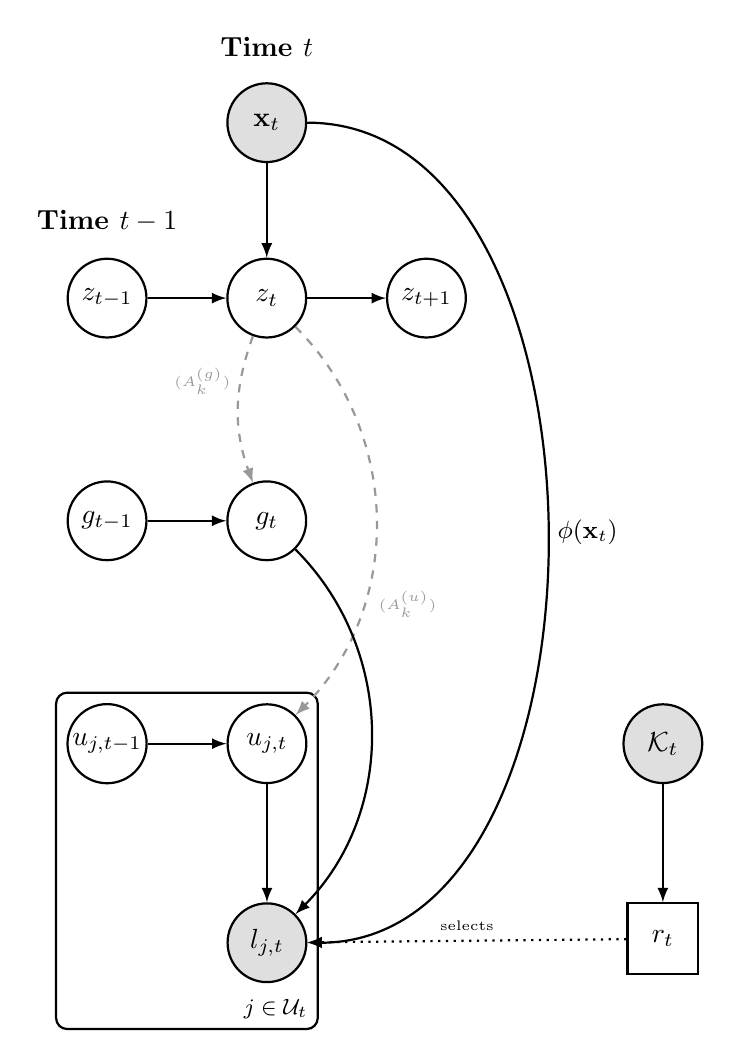
\begin{tikzpicture}[
    node distance=1.5cm and 3cm,
    >=latex,
    thick,
    latent_node/.style={latent, minimum size=1cm},
    obs_node/.style={obs, minimum size=1cm},
    action_node/.style={draw, rectangle, minimum size=0.9cm},
    param_edge/.style={->, dashed, color=gray!80}
]

% --- NODES ---

% LAYER 1: Regime (Top)
\node[latent_node] (zt_prev) {$z_{t-1}$};
\node[latent_node, right=of zt_prev] (zt) {$z_t$};
\node[latent_node, right=of zt] (zt_next) {$z_{t+1}$};

% Context (Input)
\node[obs_node, above=1.2cm of zt] (xt) {$\mathbf{x}_t$};

% LAYER 2: Shared Factor (Middle)
\node[latent_node, below=1.8cm of zt_prev] (gt_prev) {$g_{t-1}$};
\node[latent_node, right=of gt_prev] (gt) {$g_t$};

% LAYER 3: Idiosyncratic State (Bottom)
\node[latent_node, below=1.8cm of gt_prev] (ut_prev) {$u_{j,t-1}$};
\node[latent_node, right=of ut_prev] (ut) {$u_{j,t}$};

% LAYER 4: Emission/Loss
\node[obs_node, below=1.5cm of ut] (lt) {$l_{j,t}$};

% --- PLATE ---
% Represents the Universe of Experts U, not just K_t
\plate {experts} {(ut_prev)(ut)(lt)} {$j \in \mathcal{U}_t$};

% --- NEW NODES: Availability & Selection ---
% Placed to the RIGHT of the expert layer
\node[obs_node, right=4cm of ut] (Kt) {$\mathcal{K}_t$};
\node[action_node, below=1.5cm of Kt] (rt) {$r_t$};

% --- EDGES ---

% 1. Time Evolution
\edge {zt_prev} {zt};
\edge {zt} {zt_next};
\edge {gt_prev} {gt};
\edge {ut_prev} {ut};

% 2. Context Dependencies
\edge {xt} {zt};

% 3. Regime Dependencies
\draw[param_edge] (zt) to [bend right=20] node[pos=0.3, left, font=\tiny] {$(A^{(g)}_k)$} (gt);
\draw[param_edge] (zt.south east) to [bend left=45] node[pos=0.7, right, font=\tiny, xshift=2pt] {$(A^{(u)}_k)$} (ut.north east);

% 4. Emission Generation
\draw[->] (gt) to [bend left=45] (lt);
\edge {ut} {lt};

% 5. Context to Loss
\draw[->] (xt.east) to [out=0, in=0, looseness=1] node[midway, right, font=\small] {$\phi(\mathbf{x}_t)$} (lt.east);

% 6. Availability & Selection Logic
\edge {Kt} {rt}; % K_t constrains r_t
\draw[->, dotted] (rt) -- (lt) node[midway, above, font=\tiny] {selects};

% --- ANNOTATIONS ---
\node[above=0.2cm of zt_prev, font=\bfseries] {Time $t-1$};
\node[above=0.2cm of xt, font=\bfseries] {Time $t$};

\end{tikzpicture}
    \caption{Probabilistic Graphical Model of the SLDS for Partial Feedback. The plate $j \in \mathcal{U}_t$ signifies that latent states evolve for all registered experts, while $\mathcal{K}_t$ restricts the selection $r_t$.}
    \label{fig:slds_pgm_final}
\end{figure}

\section{Inference: Interacting Multiple Model (IMM) Filter}

Exact Bayesian filtering in a switching linear dynamical system is intractable in general, since the number of regime
histories \((z_1,\dots,z_t)\) grows exponentially with \(t\) (on the order of \(M^t\) for \(M\) regimes).
We therefore use the \emph{Interacting Multiple Model} (IMM) approximation, which maintains, at each time \(t\), a bank
of \(M\) regime-conditional Gaussian filters and performs a moment-matching \emph{interaction} step between regimes at
each transition. Because experts are correlated through the shared factor \(g_t\), each regime-conditional filter
operates on the joint stacked state \(\chi_t=(g_t,u_{1,t},\dots,u_{N_t,t})\), so that cross-expert correlations are
explicitly represented in the covariance of \(\chi_t\).

\paragraph{Observed history.}
For filtering, it is convenient to condition on the post-feedback interaction history up to time \(t\):
\[
    \mathcal I_t \;\coloneqq\; \bigl((\mathbf x_\tau,\Expert_\tau,G_\tau)\bigr)_{1\le \tau \le t},
    \qquad
    G_\tau \coloneqq (r_\tau,\ell_{r_\tau,\tau}).
\]
Equivalently, conditioning on \(\mathcal I_t\) means conditioning on the \(\sigma\)-field \(\sigma(\mathcal I_t)\).

\subsection{Belief-State Representation (IMM + Joint Gaussian)}

At the end of round \(t\) (after observing \(\ell_{r_t,t}\)), the filter represents the posterior over
\(\bigl(z_t,g_t,(u_{j,t})_{j\in\mathcal{U}_t}\bigr)\) via:

\begin{enumerate}
    \item \textbf{Regime probabilities.}
    \[
        b_t(k) \;\coloneqq\; \mathbb P(z_t=k \mid \mathcal I_t),
        \qquad k\in\mathcal Z.
    \]

    \item \textbf{Regime-conditional joint Gaussian state.}
    For each regime \(k\in\mathcal Z\), we maintain a Gaussian approximation for the stacked state
    \[
        \chi_t \mid \{z_t=k,\mathcal I_t\}
        \;\approx\;
        \mathcal N\!\bigl(m^{(k)}_{t\mid t},\,P^{(k)}_{t\mid t}\bigr),
    \]
    where \(\chi_t \in \mathbb R^{d_{\mathrm{state}, t}}\) is the state vector for the current registry \(\mathcal{U}_t\). The full covariance matrix
    \(P^{(k)}_{t\mid t}\) captures all cross-expert dependencies.
\end{enumerate}

\paragraph{IMM posterior approximation.}
With these quantities, the IMM approximates the joint filtering distribution as a mixture over current regimes:
\[
    p\!\left(z_t,g_t,(u_{j,t})_{j\in\mathcal{U}_t}\mid \mathcal I_t\right)
    \;\approx\;
    \sum_{k=1}^M b_t(k)\;
    \tilde p_k\!\left(g_t,(u_{j,t})_{j\in\mathcal{U}_t}\mid \mathcal I_t\right)\otimes \delta_k(z_t),
\]
where \(\tilde p_k(\cdot)\) is the Gaussian approximation characterized by the tracked moments
\(\{m^{(k)}_{t\mid t},P^{(k)}_{t\mid t}\}\).

\subsection{Step 1: Interaction (Mixing of Regime-Conditional Estimates)}

For each candidate \emph{next} regime \(k\) at time \(t+1\), the IMM interaction step constructs a mixed Gaussian initial
condition by combining the regime-conditional estimates at time \(t\).

\paragraph{Mixing weights.}
For fixed \(k\in\mathcal Z\), define
\[
    \mu_{i\mid k}
    \;\coloneqq\;
    \mathbb P(z_t=i \mid z_{t+1}=k,\mathcal I_t),
    \qquad i\in\mathcal Z.
\]

\begin{proposition}[IMM mixing weights]\label{prop:mixing_weights_star}
For each \(k\in\mathcal Z\) and \(i\in\mathcal Z\),
\[
    \mu_{i\mid k}
    \;=\;
    \frac{ \Pi_{ik}\,b_t(i)}{\bar c_k},
    \qquad
    \bar c_k \;\coloneqq\; \sum_{l=1}^M  \Pi_{lk}\,b_t(l)
    \;=\; \mathbb P(z_{t+1}=k\mid \mathcal I_t),
\]
where \( \Pi\) is the regime transition matrix.
\end{proposition}

\paragraph{Moment matching (joint form).}
For each candidate next regime \(k\in\mathcal Z\), IMM replaces the mixture over \(z_t\) by a single joint Gaussian
in the stacked state \(\chi_t\), matching its first two moments. Define the mixed mean
\[
    m^{0,(k)}_{t\mid t}
    \;\coloneqq\;
    \sum_{i=1}^M \mu_{i\mid k}\, m^{(i)}_{t\mid t}
\]
and the mixed covariance
\[
    P^{0,(k)}_{t\mid t}
    \;\coloneqq\;
    \sum_{i=1}^M \mu_{i\mid k}
    \Bigl[
        P^{(i)}_{t\mid t}
        +
        \bigl(m^{(i)}_{t\mid t}-m^{0,(k)}_{t\mid t}\bigr)
        \bigl(m^{(i)}_{t\mid t}-m^{0,(k)}_{t\mid t}\bigr)^\top
    \Bigr].
\]
These are the standard moment-matching formulas for Gaussian mixtures applied to the joint latent state defined over the registry $\mathcal{U}_t$.

\subsection{Step 2: Time Update (Prediction and Augmentation)}

The prediction step propagates the belief from $t$ to $t+1$. If new experts appear in $\Expert_{t+1}$, the state vector must first be augmented to match $\mathcal{U}_{t+1}$.

\paragraph{State Augmentation (Expert Birth).}
If $\Expert_{t+1}$ contains new experts not in $\mathcal{U}_t$, we augment the mixed moments $m^{0,(k)}_{t\mid t}$ and $P^{0,(k)}_{t\mid t}$ by appending the birth priors (Section 2.2). For each new expert $j$, we append $m^{(k)}_{u,\mathrm{birth}}$ to the mean vector and place $P^{(k)}_{u,\mathrm{birth}}$ on the corresponding diagonal block of the covariance matrix (initializing cross-covariances to zero). This yields augmented moments $\tilde{m}^{0,(k)}_{t\mid t}$ and $\tilde{P}^{0,(k)}_{t\mid t}$ of dimension matching $\mathcal{U}_{t+1}$.

\paragraph{Dynamics Application.}
Given the (possibly augmented) mixed initial condition, we apply the regime-$k$ linear dynamics. Let $A_k$ and $Q_k$ denote the transition and process-noise matrices constructed for the registry $\mathcal{U}_{t+1}$.
\begin{align}
    m^{(k)}_{t+1\mid t}
    &= A_k\, \tilde{m}^{0,(k)}_{t\mid t},
    &
    P^{(k)}_{t+1\mid t}
    &= A_k\, \tilde{P}^{0,(k)}_{t\mid t}\, A_k^\top + Q_k.
\end{align}
(Note: For experts initialized in this step, the transition $A_k$ is typically identity, simply passing the birth prior forward).

\subsection{Step 3: Measurement Update (Correction under Partial Feedback)}

At round \(t+1\), the router selects \(r_{t+1}\in\Expert_{t+1}\) and observes \(\ell_{r_{t+1},t+1}\).
(If a nonnegativity transform \(\psi\) is used, replace \(\ell_{r_{t+1},t+1}\) below by
\(\tilde\ell_{r_{t+1},t+1}\coloneqq\psi(\ell_{r_{t+1},t+1})\); the formulas are unchanged.)

Fix a regime \(k\in\mathcal Z\) and let \(r\coloneqq r_{t+1}\) be the selected expert. Define the scalar coefficients
\[
    a_{r,t+1} \;\coloneqq\; B_r^\top \phi_{t+1}\in\mathbb R^{d_g},
    \qquad
    b_{t+1} \;\coloneqq\; \phi_{t+1}\in\mathbb R^{d_\alpha}.
\]
Under \eqref{eq:observation_factor}, conditional on \(z_{t+1}=k\),
\[
    \ell_{r,t+1}
    \;=\;
    a_{r,t+1}^\top g_{t+1} + b_{t+1}^\top u_{r,t+1} + v_{r,t+1},
    \qquad v_{r,t+1}\sim\mathcal N(0,R_{k,r}).
\]

\paragraph{Regime-conditional predicted mean/variance and innovation.}
Define
\begin{align}
    \hat\ell_{t+1}^{(k)}
    &\;\coloneqq\;
    a_{r,t+1}^\top m^{(k)}_{g,t+1\mid t}
    +
    b_{t+1}^\top m^{(k)}_{u_r,t+1\mid t},
    \\
    S_{t+1}^{(k)}
    &\;\coloneqq\;
    a_{r,t+1}^\top P^{(k)}_{g,t+1\mid t} a_{r,t+1}
    +
    b_{t+1}^\top P^{(k)}_{u_r,t+1\mid t} b_{t+1}
    +
    2\,a_{r,t+1}^\top \rho^{(k)}_{r,t+1\mid t}\, b_{t+1}
    + R_{k,r},
\end{align}
and the innovation
\[
    e_{t+1}^{(k)} \;\coloneqq\; \ell_{r,t+1} - \hat\ell_{t+1}^{(k)}.
\]

\paragraph{Star Kalman gains and update for the selected expert.}
The regime-conditional gains for \(g_{t+1}\) and \(u_{r,t+1}\) are
\begin{align}
    K^{(k)}_{g,t+1}
    &\;\coloneqq\;
    \frac{P^{(k)}_{g,t+1\mid t} a_{r,t+1} + \rho^{(k)}_{r,t+1\mid t} b_{t+1}}{S_{t+1}^{(k)}}
    \in\mathbb R^{d_g},
    \\
    K^{(k)}_{u_r,t+1}
    &\;\coloneqq\;
    \frac{\rho^{(k)\top}_{r,t+1\mid t} a_{r,t+1} + P^{(k)}_{u_r,t+1\mid t} b_{t+1}}{S_{t+1}^{(k)}}
    \in\mathbb R^{d_\alpha}.
\end{align}
The filtered means update as
\begin{align}
    m^{(k)}_{g,t+1\mid t+1}
    &= m^{(k)}_{g,t+1\mid t} + K^{(k)}_{g,t+1}\, e_{t+1}^{(k)},
    \\
    m^{(k)}_{u_r,t+1\mid t+1}
    &= m^{(k)}_{u_r,t+1\mid t} + K^{(k)}_{u_r,t+1}\, e_{t+1}^{(k)},
\end{align}
and the filtered covariances (including the star cross-covariance) update as
\begin{align}
    P^{(k)}_{g,t+1\mid t+1}
    &= P^{(k)}_{g,t+1\mid t} - K^{(k)}_{g,t+1}\, S_{t+1}^{(k)}\, K^{(k)\top}_{g,t+1},
    \\
    P^{(k)}_{u_r,t+1\mid t+1}
    &= P^{(k)}_{u_r,t+1\mid t} - K^{(k)}_{u_r,t+1}\, S_{t+1}^{(k)}\, K^{(k)\top}_{u_r,t+1},
    \\
    \rho^{(k)}_{r,t+1\mid t+1}
    &= \rho^{(k)}_{r,t+1\mid t} - K^{(k)}_{g,t+1}\, S_{t+1}^{(k)}\, K^{(k)\top}_{u_r,t+1}.
\end{align}
These are exactly the block updates obtained by applying a Kalman update to the joint Gaussian state
\((g_{t+1},u_{r,t+1})\) with scalar observation vector \((a_{r,t+1},b_{t+1})\), followed by maintaining the star
structure.

\paragraph{Unselected experts (indirect star update).}
For each \(j\neq r\) (where \(j \in \mathcal{U}_{t+1}\)), there is no direct measurement of \(\ell_{j,t+1}\). Under the star approximation, we optionally propagate the information gained about \(g_{t+1}\) to \((u_{j,t+1},\rho_{j,t+1})\) by keeping the prior conditional
\(u_{j,t+1}\mid g_{t+1}\) and updating only the marginal of \(g_{t+1}\). For each \(j\neq r\),
\begin{align}
    m^{(k)}_{u_j,t+1\mid t+1}
    &=
    m^{(k)}_{u_j,t+1\mid t}
    +
    \rho^{(k)\top}_{j,t+1\mid t}\,
    \bigl(P^{(k)}_{g,t+1\mid t}\bigr)^{-1}
    \bigl(m^{(k)}_{g,t+1\mid t+1}-m^{(k)}_{g,t+1\mid t}\bigr),
    \\
    P^{(k)}_{u_j,t+1\mid t+1}
    &=
    P^{(k)}_{u_j,t+1\mid t}
    +
    \rho^{(k)\top}_{j,t+1\mid t}\,
    \bigl(P^{(k)}_{g,t+1\mid t}\bigr)^{-1}
    \bigl(P^{(k)}_{g,t+1\mid t+1}-P^{(k)}_{g,t+1\mid t}\bigr)
    \bigl(P^{(k)}_{g,t+1\mid t}\bigr)^{-1}
    \rho^{(k)}_{j,t+1\mid t},
    \\
    \rho^{(k)}_{j,t+1\mid t+1}
    &=
    P^{(k)}_{g,t+1\mid t+1}\,
    \bigl(P^{(k)}_{g,t+1\mid t}\bigr)^{-1}\,
    \rho^{(k)}_{j,t+1\mid t}.
\end{align}
If one prefers a cheaper update, one may skip this indirect step and simply set
\(
m^{(k)}_{u_j,t+1\mid t+1}=m^{(k)}_{u_j,t+1\mid t},
P^{(k)}_{u_j,t+1\mid t+1}=P^{(k)}_{u_j,t+1\mid t},
\rho^{(k)}_{j,t+1\mid t+1}=\rho^{(k)}_{j,t+1\mid t}
\)
for \(j\neq r\).

\subsection{Step 4: Regime Probability Update}

Finally, we update regime probabilities using the likelihood of the observed loss under each regime hypothesis. For each
\(k\in\mathcal Z\), define the Gaussian likelihood (density value)
\[
    \Lambda_{t+1}^{(k)}
    \;\coloneqq\;
    \mathcal N\!\bigl(
        \ell_{r,t+1};
        \hat{\ell}_{t+1}^{(k)},
        S_{t+1}^{(k)}
    \bigr).
\]
Using the predicted regime probabilities \(\bar c_k=\sum_{l=1}^M  \Pi_{lk} b_t(l)\) from
Proposition~\ref{prop:mixing_weights_star}, Bayes' rule yields
\[
    b_{t+1}(k)
    \;\coloneqq\;
    \mathbb P(z_{t+1}=k \mid \mathcal I_{t+1})
    \;=\;
    \frac{\Lambda_{t+1}^{(k)} \, \bar c_k}{\sum_{l=1}^M \Lambda_{t+1}^{(l)} \, \bar c_l},
    \qquad k\in\mathcal Z.
\]

\begin{remark}[What is approximated: IMM]\label{rem:imm_approx}
For \(M=1\), IMM reduces to a single regime-conditional Kalman filter; for \(M\ge 2\), IMM introduces:
\begin{enumerate}[label=(\roman*)]
    \item \textbf{Regime-history truncation:} the exact filtering distribution is a mixture over all regime histories
    \((z_1,\dots,z_t)\) (size \(M^t\)); IMM retains only \(M\) components indexed by \(z_t\).
    \item \textbf{Inter-regime moment matching:} for each candidate next regime \(k\), the mixed prior over \(z_t\) is a
    mixture of Gaussians; IMM replaces it by a single Gaussian with matched moments.
\end{enumerate}
Thus the method preserves regime probabilities and the tracked first/second moments of the joint latent state by
construction, but does not in general preserve higher-order moments nor exact regime-history dependencies.
\end{remark}

\section{Selection Policy}

At decision time $t+1$, the router observes
\[
    H_{t+1} \;=\; (\mathcal I_t,\mathbf x_{t+1},\Expert_{t+1}),
\]
i.e., the post-feedback history up to $t$, the current context $\mathbf x_{t+1}$ (hence $\phi_{t+1}$), and the available
expert set $\Expert_{t+1}$. Based on $H_{t+1}$, the router must choose an expert index
\(
    r_{t+1}\in\Expert_{t+1}.
\)

Recall that if expert $j$ were selected at time $t+1$, the one-step total cost would be
\[
    C_{j,t+1} \;\coloneqq\; \ell_{j,t+1} + \beta_j,
\]
where $\beta_j\ge 0$ is deterministic and known at decision time.

A purely risk-neutral, myopic rule would minimize the conditional mean
\(
    \mathbb E[C_{j,t+1}\mid H_{t+1}]
\)
over $j\in\Expert_{t+1}$. Below we use a one-step \emph{risk-sensitive} criterion that additionally depends on the
conditional variance of $C_{j,t+1}$ given $H_{t+1}$.

\subsection{One-step Forecast under IMM + Star (Predictive Mean)}

Fix an expert $j\in\mathcal{U}_{t+1}$. Under the IMM filter, the \emph{predicted} regime probabilities for $z_{t+1}$ given the
information available at the end of round $t$ are
\[
    \bar c_k
    \;\coloneqq\;
    \mathbb P(z_{t+1}=k\mid \mathcal I_t),
    \qquad k\in\mathcal Z.
\]
(Note: We use $\bar c_k$ for the predicted regime probability to distinguish it from the filtered belief $b_t(k)$).

Under the Option~A factorization with joint Gaussian filtering, the regime-$k$ time update at round $t+1$ provides the
predictive moments $(m^{(k)}_{t+1\mid t},P^{(k)}_{t+1\mid t})$ for the stacked state
$\chi_{t+1}$ (defined over the registry $\mathcal{U}_{t+1}$).

After observing $\mathbf x_{t+1}$ (and computing features $\phi_{t+1}$), define the global factor loading coefficient:
\[
    a_{j,t+1} \;\coloneqq\; B_j^\top \phi_{t+1}\in\mathbb R^{d_g}.
\]
Under the linear-Gaussian emission \eqref{eq:observation_factor}, the regime-conditional predictive distribution of the
loss is Gaussian:
\[
    \ell_{j,t+1}\mid\{z_{t+1}=k,H_{t+1}\}
    \;\approx\;
    \mathcal N\!\bigl(\mu^{(k)}_{j,t+1\mid t},\,\sigma^{2,(k)}_{j,t+1\mid t}\bigr),
\]
with
\begin{align}
    \mu^{(k)}_{j,t+1\mid t}
    &\;\coloneqq\;
    a_{j,t+1}^\top m^{(k)}_{g,t+1\mid t} + \phi_{t+1}^\top m^{(k)}_{u_j,t+1\mid t},
    \label{eq:sel_mu_regime}
    \\
    \sigma^{2,(k)}_{j,t+1\mid t}
    &\;\coloneqq\;
    h_{j,t+1}^\top P^{(k)}_{t+1\mid t} h_{j,t+1}
    + R_{k,j}.
    \label{eq:sel_var_regime}
\end{align}
(Here $h_{j,t+1}$ is the full observation vector constructed from $a_{j,t+1}$ and $\phi_{t+1}$ as defined in Section~\ref{sec:observation-partial}).

Therefore, the IMM+joint approximation induces the following one-step predictive mixture for $\ell_{j,t+1}$:
\[
    \mathbb P(\ell_{j,t+1}\mid H_{t+1})
    \;\approx\;
    \sum_{k=1}^M \bar c_k\,
    \mathcal N\!\bigl(\cdot;\mu^{(k)}_{j,t+1\mid t},\,\sigma^{2,(k)}_{j,t+1\mid t}\bigr).
\]
Under squared loss for predicting $\ell_{j,t+1}$, the optimal point predictor is the conditional mean, which we
approximate by
\begin{equation}
    \label{eq:sel_mean_mix}
    \widehat{\ell}_{j,t+1\mid t}
    \;\coloneqq\;
    \mathbb E[\ell_{j,t+1}\mid H_{t+1}]
    \;\approx\;
    \sum_{k=1}^M \bar c_k\, \mu^{(k)}_{j,t+1\mid t}.
\end{equation}

\paragraph{Modeling note (nonnegativity).}
If the filter is run on a transformed observation $\tilde\ell_{j,t}=\psi(\ell_{j,t})$ (e.g.\ $\psi(x)=\log(x+\varepsilon)$),
then all formulas above apply with $\ell$ replaced by $\tilde\ell$ (and $\mu,\sigma^2$ interpreted on the transformed
scale). Converting the forecast back to the original loss requires pushing the Gaussian predictive law through
$\psi^{-1}$ (closed form for $\psi(x)=\log(x+\varepsilon)$; otherwise delta method / Monte Carlo).

\subsection{Predictive Variance and Epistemic Uncertainty}

Define the conditional predictive variance
\[
    \hat\sigma^2_{j,t+1\mid t}
    \;\coloneqq\;
    \Var(\ell_{j,t+1}\mid H_{t+1}),
\]
and note that since $\beta_j$ is deterministic,
\[
    \Var(C_{j,t+1}\mid H_{t+1})=\Var(\ell_{j,t+1}\mid H_{t+1})=\hat\sigma^2_{j,t+1\mid t}.
\]

\begin{proposition}[Predictive variance decomposition]\label{prop:total_variance}
For each expert $j\in\mathcal{U}_{t+1}$,
\begin{equation}
    \label{eq:total_variance}
    \hat\sigma^2_{j,t+1\mid t}
    \;\approx\;
    \sum_{k=1}^M \bar c_k\, \sigma^{2,(k)}_{j,t+1\mid t}
    \;+\;
    \sum_{k=1}^M \bar c_k\,
    \bigl(\mu^{(k)}_{j,t+1\mid t} - \widehat{\ell}_{j,t+1\mid t}\bigr)^2,
\end{equation}
where $\widehat{\ell}_{j,t+1\mid t}$ is defined in \eqref{eq:sel_mean_mix}.
\end{proposition}

\begin{proof}
Apply the law of total variance with $Y=\ell_{j,t+1}$ and $Z=z_{t+1}$, conditioning on $H_{t+1}$:
\[
    \Var(Y\mid H_{t+1})
    =
    \mathbb E\!\bigl[\Var(Y\mid Z,H_{t+1})\mid H_{t+1}\bigr]
    +
    \Var\!\bigl(\mathbb E[Y\mid Z,H_{t+1}]\mid H_{t+1}\bigr).
\]
Under $Z=k$, the (approximate) conditional mean and variance are $\mu^{(k)}_{j,t+1\mid t}$ and
$\sigma^{2,(k)}_{j,t+1\mid t}$ from \eqref{eq:sel_mu_regime}--\eqref{eq:sel_var_regime}. Replacing
$\mathbb P(Z=k\mid H_{t+1})$ by the IMM predictor $\bar c_k=\mathbb P(Z=k\mid\mathcal I_t)$ yields
\eqref{eq:total_variance}.
\end{proof}

\subsection{Cost-Sensitive Selection Rule}

For each available expert $j\in\Expert_{t+1}$, define the risk-adjusted score
\[
    J_{j,t+1}
    \;\coloneqq\;
    \widehat{\ell}_{j,t+1\mid t}
    + \beta_j
    + \lambda\sqrt{\hat\sigma^2_{j,t+1\mid t}},
\]
where $\lambda\in\mathbb R$ is a user-specified risk parameter. The router selects
\begin{equation}
    \label{eq:policy}
    r_{t+1}^\star
    \;\in\;
    \arg\min_{j\in\Expert_{t+1}} J_{j,t+1}.
\end{equation}
For $\lambda=0$, this reduces to a myopic mean-cost rule; $\lambda>0$ penalizes predictive uncertainty.

\begin{proposition}[Tail-control interpretation via Cantelli]
\label{prop:cantelli}
Fix $t$ and condition on $H_{t+1}$. For any expert $j\in\Expert_{t+1}$, let
\[
    m_{j} \coloneqq \mathbb E[C_{j,t+1}\mid H_{t+1}],
    \qquad
    s_{j}^2 \coloneqq \Var(C_{j,t+1}\mid H_{t+1}).
\]
Then for any $\lambda>0$,
\[
    \mathbb P\!\left(
        C_{j,t+1} \le m_j + \lambda s_j \,\middle|\, H_{t+1}
    \right)
    \;\ge\;
    \frac{\lambda^2}{1+\lambda^2}.
\]
Equivalently,
\(
    \mathbb P\!\left(C_{j,t+1} - m_j \ge \lambda s_j \mid H_{t+1}\right)
    \le \frac{1}{1+\lambda^2}.
\)
\end{proposition}

\begin{proof}
Cantelli's inequality applied conditionally on $H_{t+1}$:
\(
    \mathbb P(X-\mathbb E[X]\ge a)\le \Var(X)/(\Var(X)+a^2)
\)
with $X=C_{j,t+1}$ and $a=\lambda s_j$.
\end{proof}

\noindent
\emph{Implication.}
For $\lambda>0$, the threshold $m_j+\lambda s_j$ is exceeded with conditional probability at most $1/(1+\lambda^2)$.
Thus, minimizing $J_{j,t+1}$ can be read as selecting the expert with the smallest
mean--standard-deviation upper envelope of the next-step cost, where the envelope level is controlled by $\lambda$.

\begin{remark}[One-step risk-adjusted Bayes action]\label{rem:one_step_bayes_risk}
Fix $t$ and condition on $H_{t+1}$. Define the local risk functional
\[
    \mathcal R^\lambda_{t+1}(Y)
    \;\coloneqq\;
    \mathbb E[Y\mid H_{t+1}] + \lambda\sqrt{\Var(Y\mid H_{t+1})},
    \qquad \lambda\in\mathbb R.
\]
Then \eqref{eq:policy} is exactly
\[
    r_{t+1}^\star\in\arg\min_{j\in\Expert_{t+1}} \mathcal R^\lambda_{t+1}\!\bigl(C_{j,t+1}\bigr).
\]
\end{remark}

\paragraph{Regime-Dependent Risk Aversion.}
A static risk parameter $\lambda$ may be insufficient for environments with distinct safety requirements (e.g., ``routine'' vs.\ ``critical'' regimes). We allow the user to specify a vector of risk parameters $\bm{\lambda} = (\lambda^{(1)}, \dots, \lambda^{(M)})$, where $\lambda^{(k)}$ encodes the risk tolerance in regime $k$.

The effective risk parameter at time $t$ is the expected risk aversion under the current belief state:
\[
    \bar{\lambda}_t \;\coloneqq\; \sum_{k=1}^M b_t(k) \, \lambda^{(k)}.
\]
The scoring rule \eqref{eq:policy} is updated to use $\bar{\lambda}_t$. This allows the router to dynamically become more conservative when the IMM filter detects a shift to a volatile or high-stakes regime.

\section{Parameter Optimization}
\label{sec:param-opt}

Under Option~A with star covariance tracking, the latent variables are the regime sequence
$Z_{1:T}=(z_t)_{t=1}^T$, the shared factor $G_{1:T}=(g_t)_{t=1}^T$, and the idiosyncratic states
$U_{1:T}=\{u_{j,t}\}_{j\in\mathcal{U}_T,\,1\le t\le T}$ (defined for the set of all experts $\mathcal{U}_T$ encountered by the end of the horizon).
We treat the feature map $\phi:\mathcal X\to\mathbb R^{d_\alpha}$ and the loadings $(B_j)_{j\in\mathcal{U}_T}$
as \emph{fixed} (not learned), and learn the remaining SLDS parameters.

\paragraph{Parameters.}
We collect the learnable parameters in
\[
    \Theta
    \;\coloneqq\;
    \Bigl(
         \Pi,\ \mu^0,\ (A^{(g)}_k,Q^{(g)}_k)_{k=1}^M,\ (A^{(u)}_k,Q^{(u)}_k)_{k=1}^M,\
        (R_{k,j})_{\substack{k=1,\dots,M\\ j\in\mathcal{U}_T}},\ \text{initial/birth priors}
    \Bigr),
\]
where $ \Pi\in[0,1]^{M\times M}$ is the regime transition matrix, $\mu^0$ is the initial regime distribution,
and $(A^{(g)}_k,Q^{(g)}_k)$ and $(A^{(u)}_k,Q^{(u)}_k)$ are the regime-dependent dynamics matrices in
\eqref{eq:global_factor_transition}--\eqref{eq:idiosyncratic_transition}.
The scalars $R_{k,j}>0$ are the observation-noise variances in \eqref{eq:observation_factor}.

\paragraph{Observed data and history.}
We observe a single scalar loss per round (bandit feedback):
\[
    \mathbf D \;\coloneqq\; \{(\mathbf x_t,\Expert_t,r_t,\ell_{r_t,t})\}_{t=1}^T,
    \qquad
    \mathcal I_t \;\coloneqq\; \bigl((\mathbf x_\tau,\Expert_\tau,G_\tau)\bigr)_{1\le \tau\le t},
    \ \ G_\tau=(r_\tau,\ell_{r_\tau,\tau}).
\]

\subsection{Conditional (Controlled) Maximum Likelihood Objective}

We treat $(\Expert_t,r_t)$ as exogenous controls (censoring only), and maximize the conditional marginal likelihood of
the observed losses. The conditional log-likelihood is
\begin{equation}
\label{eq:MLE_objective}
    \mathcal J(\Theta)
    \;\coloneqq\;
    \sum_{t=1}^T
    \log p_\Theta(\ell_{r_t,t}\mid \mathcal I_{t-1},\mathbf x_t,\Expert_t,r_t).
\end{equation}

\paragraph{IMM predictive mixture used in practice.}
Exact SLDS prediction is intractable for $M\ge 2$. Using IMM, we approximate the predictive density at time $t$ by
\begin{equation}
\label{eq:imm_predictive_density}
    \tilde p_\Theta^{\mathrm{IMM}}(\ell_{r_t,t}\mid \mathcal I_{t-1},\mathbf x_t,\Expert_t,r_t)
    \;\coloneqq\;
    \sum_{k=1}^M \bar c_t(k)\,\Lambda_t^{(k)},
\end{equation}
where $\bar c_t(k)=\mathbb P_\Theta(z_t=k\mid \mathcal I_{t-1})$ is the one-step regime predictor and
$\Lambda_t^{(k)}$ is the regime-$k$ scalar Gaussian likelihood under the star predictor.

Let $\phi_t\coloneqq \phi(\mathbf x_t)$ and $r\coloneqq r_t$.
Define $a_{r,t}\coloneqq B_r^\top \phi_t\in\mathbb R^{d_g}$.
Under regime $k$, the star predictor provides $(m^{(k)}_{g,t\mid t-1},P^{(k)}_{g,t\mid t-1})$,
$(m^{(k)}_{u_r,t\mid t-1},P^{(k)}_{u_r,t\mid t-1})$, and $\rho^{(k)}_{r,t\mid t-1}=\Cov(g_t,u_{r,t}\mid z_t=k,\mathcal I_{t-1})$.
Then
\[
    \Lambda_t^{(k)}
    =
    \mathcal N\!\bigl(\ell_{r_t,t};\ \mu^{(k)}_{r,t\mid t-1},\ \sigma^{2,(k)}_{r,t\mid t-1}\bigr),
\]
with
\begin{align}
\label{eq:ll_mu_star}
    \mu^{(k)}_{r,t\mid t-1}
    &\;\coloneqq\;
    a_{r,t}^\top m^{(k)}_{g,t\mid t-1} + \phi_t^\top m^{(k)}_{u_r,t\mid t-1},
    \\
\label{eq:ll_var_star}
    \sigma^{2,(k)}_{r,t\mid t-1}
    &\;\coloneqq\;
    a_{r,t}^\top P^{(k)}_{g,t\mid t-1} a_{r,t}
    + \phi_t^\top P^{(k)}_{u_r,t\mid t-1} \phi_t
    + 2\,a_{r,t}^\top \rho^{(k)}_{r,t\mid t-1} \phi_t
    + R_{k,r}.
\end{align}

Accordingly the objective actually evaluated is the IMM surrogate log-likelihood
\begin{equation}
\label{eq:imm_surrogate_objective}
    \tilde{\mathcal J}_{\mathrm{IMM}}(\Theta)
    \;\coloneqq\;
    \sum_{t=1}^T
    \log \tilde p_\Theta^{\mathrm{IMM}}(\ell_{r_t,t}\mid \mathcal I_{t-1},\mathbf x_t,\Expert_t,r_t).
\end{equation}

\subsection{Generalized EM with IMM + Star Smoothing}

We use a generalized EM procedure: an IMM forward filter and an approximate backward smoother yield an approximate
posterior $q^{(m)}$ under $\Theta^{(m)}$, and the M-step increases the corresponding EM auxiliary functional
\[
    Q(\Theta;\Theta^{(m)})
    \;\coloneqq\;
    \mathbb E_{q^{(m)}}\!\left[\log p_\Theta(\mathbf D,Z_{1:T},G_{1:T},U_{1:T})\right].
\]

\paragraph{E-step outputs.}
The IMM smoother provides approximate smoothed regime marginals and pairwise marginals:
\[
    \gamma_t^{(k)} \approx \mathbb P(z_t=k\mid \mathcal I_T),
    \qquad
    \xi_t^{(i,k)} \approx \mathbb P(z_{t-1}=i,z_t=k\mid \mathcal I_T),
\]
and (regime-conditional) Gaussian star moments for $(g_t,u_{j,t})$ for any $j \in \mathcal{U}_t$:
\[
    (g_t,u_{j,t})\mid\{z_t=k,\mathcal I_T\}
    \approx
    \mathcal N\!\left(
        \begin{bmatrix} m^{(k)}_{g,t\mid T}\\ m^{(k)}_{u_j,t\mid T}\end{bmatrix},
        \begin{bmatrix}
            P^{(k)}_{g,t\mid T} & \rho^{(k)}_{j,t\mid T}\\
            \rho^{(k)\top}_{j,t\mid T} & P^{(k)}_{u_j,t\mid T}
        \end{bmatrix}
    \right),
\]
together with lag-one covariances for the dynamics:
\[
    P^{(k)}_{g,t,t-1\mid T}\approx \Cov(g_t,g_{t-1}\mid z_t=k,\mathcal I_T),
    \qquad
    P^{(k)}_{u_j,t,t-1\mid T}\approx \Cov(u_{j,t},u_{j,t-1}\mid z_t=k,\mathcal I_T).
\]

\subsection{M-step (closed-form updates)}

\paragraph{Initial regime distribution.}
\[
    \mu^{0,(m+1)}_k \;=\; \gamma_1^{(k)}.
\]

\paragraph{Regime transitions.}
For each $i,k\in\mathcal Z$,
\[
     \Pi_{ik}^{(m+1)} \;=\;
    \frac{\sum_{t=2}^T \xi_t^{(i,k)}}{\sum_{t=2}^T \sum_{k'=1}^M \xi_t^{(i,k')}}.
\]

\paragraph{Factor dynamics $(A^{(g)}_k,Q^{(g)}_k)$.}
For each $k\in\mathcal Z$, define the weighted sufficient statistics
\begin{align*}
    S^{(k)}_{11,g} &\coloneqq \sum_{t=2}^T \gamma_t^{(k)}\,
    \mathbb E[g_{t-1}g_{t-1}^\top \mid z_t=k,\mathcal I_T],\\
    S^{(k)}_{10,g} &\coloneqq \sum_{t=2}^T \gamma_t^{(k)}\,
    \mathbb E[g_{t}g_{t-1}^\top \mid z_t=k,\mathcal I_T],\\
    S^{(k)}_{00,g} &\coloneqq \sum_{t=2}^T \gamma_t^{(k)}\,
    \mathbb E[g_{t}g_{t}^\top \mid z_t=k,\mathcal I_T].
\end{align*}
Under the Gaussian approximation,
\[
    \mathbb E[g_t g_t^\top \mid z_t=k,\mathcal I_T]
    = P^{(k)}_{g,t\mid T} + m^{(k)}_{g,t\mid T} m^{(k)\top}_{g,t\mid T},
\qquad
    \mathbb E[g_t g_{t-1}^\top \mid z_t=k,\mathcal I_T]
    = P^{(k)}_{g,t,t-1\mid T} + m^{(k)}_{g,t\mid T} m^{(k)\top}_{g,t-1\mid T}.
\]
If $S^{(k)}_{11,g}$ is invertible, the M-step updates are
\[
    A^{(g),(m+1)}_k \;=\; S^{(k)}_{10,g}\bigl(S^{(k)}_{11,g}\bigr)^{-1},
\]
and
\[
    Q^{(g),(m+1)}_k
    \;=\;
    \frac{1}{\sum_{t=2}^T \gamma_t^{(k)}}
    \Bigl(S^{(k)}_{00,g} - A^{(g),(m+1)}_k S^{(k)\top}_{10,g}\Bigr),
\]
followed by symmetrization/projection onto $\mathbb S_{+}^{d_g}$ if needed.

\paragraph{Idiosyncratic dynamics $(A^{(u)}_k,Q^{(u)}_k)$.}
Similarly, for each $k\in\mathcal Z$ define the sufficient statistics by summing over all experts in the final registry $\mathcal{U}_T$. Note that for each expert $j \in \mathcal{U}_T$, the latent state $u_{j,t}$ is defined only for $t \ge \tau_j$ (the expert's birth time).
\begin{align*}
    S^{(k)}_{11,u} &\coloneqq \sum_{j\in\mathcal{U}_T}\sum_{t=\tau_j+1}^T \gamma_t^{(k)}\,
    \mathbb E[u_{j,t-1}u_{j,t-1}^\top \mid z_t=k,\mathcal I_T],\\
    S^{(k)}_{10,u} &\coloneqq \sum_{j\in\mathcal{U}_T}\sum_{t=\tau_j+1}^T \gamma_t^{(k)}\,
    \mathbb E[u_{j,t}u_{j,t-1}^\top \mid z_t=k,\mathcal I_T],\\
    S^{(k)}_{00,u} &\coloneqq \sum_{j\in\mathcal{U}_T}\sum_{t=\tau_j+1}^T \gamma_t^{(k)}\,
    \mathbb E[u_{j,t}u_{j,t}^\top \mid z_t=k,\mathcal I_T].
\end{align*}
Then (when $S^{(k)}_{11,u}$ is invertible)
\[
    A^{(u),(m+1)}_k \;=\; S^{(k)}_{10,u}\bigl(S^{(k)}_{11,u}\bigr)^{-1},
\]
and
\[
    Q^{(u),(m+1)}_k
    \;=\;
    \frac{1}{\sum_{j\in\mathcal{U}_T}\sum_{t=\tau_j+1}^T \gamma_t^{(k)}}
    \Bigl(S^{(k)}_{00,u} - A^{(u),(m+1)}_k S^{(k)\top}_{10,u}\Bigr),
\]
with symmetrization/projection if needed.

\paragraph{Observation noise $R_{k,j}$.}
For each pair $(k,j)$, use only times where expert $j$ was selected ($r_t=j$). Let $\phi_t=\phi(\mathbf x_t)$ and
$a_{j,t}=B_j^\top \phi_t$. Define the star-posterior predictive mean of the linear form
$a_{j,t}^\top g_t + \phi_t^\top u_{j,t}$ under regime $k$ as
\[
    \hat y^{(k)}_{j,t}
    \;\coloneqq\;
    a_{j,t}^\top m^{(k)}_{g,t\mid T} + \phi_t^\top m^{(k)}_{u_j,t\mid T},
\]
and its variance as
\[
    \hat v^{(k)}_{j,t}
    \;\coloneqq\;
    a_{j,t}^\top P^{(k)}_{g,t\mid T} a_{j,t}
    + \phi_t^\top P^{(k)}_{u_j,t\mid T} \phi_t
    + 2\,a_{j,t}^\top \rho^{(k)}_{j,t\mid T} \phi_t.
\]
Then the M-step update is
\[
    R_{k,j}^{(m+1)}
    \;=\;
    \frac{\sum_{t:\,r_t=j}\gamma_t^{(k)}\Bigl[(\ell_{j,t}-\hat y^{(k)}_{j,t})^2+\hat v^{(k)}_{j,t}\Bigr]}
         {\sum_{t:\,r_t=j}\gamma_t^{(k)}}.
\]
If a transform $\tilde\ell_{j,t}=\psi(\ell_{j,t})$ is used in the emission, replace $\ell_{j,t}$ by $\tilde\ell_{j,t}$
everywhere in this update.

\begin{remark}[Identifiability under bandit feedback]
Because only the selected expert is observed, $R_{k,j}$ and any untied expert-specific parameters are weakly identified
for rarely queried experts. In practice, one often ties parameters (e.g.\ $R_{k,j}\equiv R_k$), uses informative priors,
and/or enforces exploration to keep the system identifiable.
\end{remark}

\section{Extension: Full-Information Expert Feedback}
\label{sec:full-info}

In the main development, the router observes at each time $t$ only the loss of the selected expert $r_t$, leading to a
censored (bandit-style) feedback model. In some applications---e.g.\ when all experts are implemented as models that can
be evaluated offline once the ground-truth outcome is revealed---it is natural to assume a \emph{full-information} setting:
after each decision epoch, the losses of \emph{all available} experts can be computed from the realized outcome, regardless
of which expert was queried for decision-making.

This section formalizes the full-information feedback model and the corresponding modifications to SLDS--IMM inference and
to the routing problem.

\subsection{Feedback model with full expert losses}

We retain the generative model of Sections~\ref{sec:slds}--\ref{sec:imm} together with the shared-factor reliability model
(Option~A with star covariance tracking) from Section~\ref{sec:observation-partial}. In particular, at each $t\ge 1$ we
write $\phi_t\coloneqq \phi(\mathbf x_t)\in\mathbb R^{d_\alpha}$ and, conditionally on $z_t=k$, for every $j\in\mathcal{U}_t$ (the current registry),
\begin{equation}
\label{eq:fullinfo_emission}
    \ell_{j,t}
    \;=\;
    \phi_t^\top\!\bigl(B_j g_t + u_{j,t}\bigr)
    +
    v_{j,t},
    \qquad
    v_{j,t}\sim\mathcal N(0,R_{k,j}),
\end{equation}
with $(v_{j,t})_{j,t}$ independent across $j$ and $t$, and independent of the latent states conditional on
$(z_t,g_t,(u_{j,t})_{j\in\mathcal{U}_t})$. (If a monotone transform $\psi$ is used, \eqref{eq:fullinfo_emission} is understood
as applying to $\tilde{\ell}_{j,t}=\psi(\ell_{j,t})$.)

\begin{figure}[h]
    \centering
    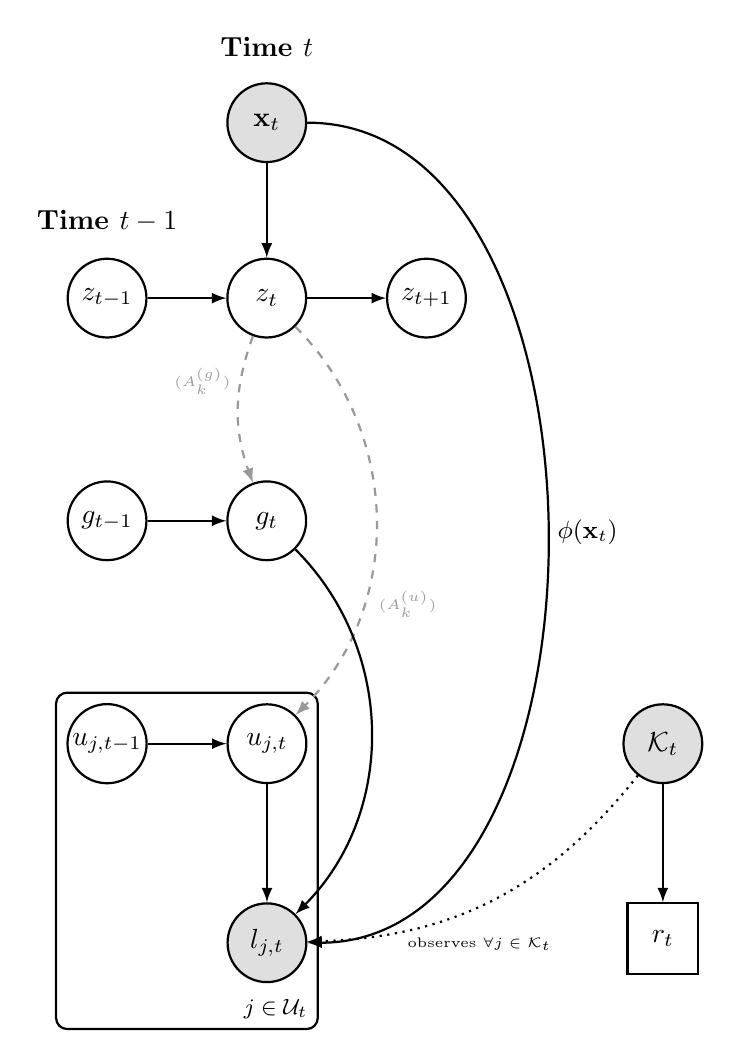
\begin{tikzpicture}[
    node distance=1.5cm and 3cm,
    >=latex,
    thick,
    latent_node/.style={latent, minimum size=1cm},
    obs_node/.style={obs, minimum size=1cm},
    action_node/.style={draw, rectangle, minimum size=0.9cm},
    param_edge/.style={->, dashed, color=gray!80}
]

% --- NODES ---

% LAYER 1: Regime (Top)
\node[latent_node] (zt_prev) {$z_{t-1}$};
\node[latent_node, right=of zt_prev] (zt) {$z_t$};
\node[latent_node, right=of zt] (zt_next) {$z_{t+1}$};

% Context (Input)
\node[obs_node, above=1.2cm of zt] (xt) {$\mathbf{x}_t$};

% LAYER 2: Shared Factor (Middle)
\node[latent_node, below=1.8cm of zt_prev] (gt_prev) {$g_{t-1}$};
\node[latent_node, right=of gt_prev] (gt) {$g_t$};

% LAYER 3: Idiosyncratic State (Bottom)
\node[latent_node, below=1.8cm of gt_prev] (ut_prev) {$u_{j,t-1}$};
\node[latent_node, right=of ut_prev] (ut) {$u_{j,t}$};

% LAYER 4: Emission/Loss
\node[obs_node, below=1.5cm of ut] (lt) {$l_{j,t}$};

% --- PLATE ---
\plate {experts} {(ut_prev)(ut)(lt)} {$j \in \mathcal{U}_t$};

% --- NEW NODES: Availability & Selection ---
% Placed to the RIGHT (same as previous graph for consistency)
\node[obs_node, right=4cm of ut] (Kt) {$\mathcal{K}_t$};
\node[action_node, below=1.5cm of Kt] (rt) {$r_t$};

% --- EDGES ---

% 1. Time Evolution
\edge {zt_prev} {zt};
\edge {zt} {zt_next};
\edge {gt_prev} {gt};
\edge {ut_prev} {ut};

% 2. Context Dependencies
\edge {xt} {zt};

% 3. Regime Dependencies
\draw[param_edge] (zt) to [bend right=20] node[pos=0.3, left, font=\tiny] {$(A^{(g)}_k)$} (gt);
\draw[param_edge] (zt.south east) to [bend left=45] node[pos=0.7, right, font=\tiny, xshift=2pt] {$(A^{(u)}_k)$} (ut.north east);

% 4. Emission Generation
\draw[->] (gt) to [bend left=45] (lt);
\edge {ut} {lt};

% 5. Context to Loss
\draw[->] (xt.east) to [out=0, in=0, looseness=1] node[midway, right, font=\small] {$\phi(\mathbf{x}_t)$} (lt.east);

% 6. Full Feedback Logic (The Change)
\edge {Kt} {rt}; % K_t still constrains the decision space

% NO EDGE from r_t to l_{j,t}.
% Instead, K_t determines observability directly.
\draw[->, dotted] (Kt) to [bend left=25] node[midway, below, font=\tiny, xshift=-5pt, yshift=-10pt] {observes $\forall j \in \mathcal{K}_t$} (lt);

% --- ANNOTATIONS ---
\node[above=0.2cm of zt_prev, font=\bfseries] {Time $t-1$};
\node[above=0.2cm of xt, font=\bfseries] {Time $t$};

\end{tikzpicture}
    \caption{PGM for the \textbf{Full Feedback} setting. Unlike the bandit case, the selection $r_t$ does not gate the observation; losses are observed for all available experts in $\mathcal{K}_t$.}
    \label{fig:slds_pgm_full_feedback}
\end{figure}


\paragraph{Decision-time information and full feedback.}
At time $t$, before observing any losses at $t$, the router observes
\[
    H_t^{\mathrm{full}}
    \;\coloneqq\;
    \bigl(\mathcal I_{t-1}^{\mathrm{full}},\,\mathbf x_t,\,\Expert_t\bigr),
\]
where the (post-feedback) history up to $t-1$ is
\[
    \mathcal I_{t-1}^{\mathrm{full}}
    \;\coloneqq\;
    \bigl((\mathbf x_\tau,\Expert_\tau,G_\tau)\bigr)_{1\le \tau\le t-1},
    \qquad
    \mathcal I_{0}^{\mathrm{full}} \text{ empty.}
\]
The router then selects $r_t\in\Expert_t$ (as in the base model). After the outcome $y_t$ is revealed, the system provides
the \emph{full panel} of losses for all available experts:
\[
    \ell_{j,t}=\mathcal L\bigl(f_j(\mathbf x_t),y_t\bigr),
    \qquad j\in\Expert_t.
\]
We encode the post-decision feedback as
\[
    G_t
    \;\coloneqq\;
    \bigl(r_t,\ (\ell_{j,t})_{j\in\Expert_t}\bigr),
\]
and define the full-information filtration by
\[
    \mathcal F_t \;\coloneqq\; \sigma(H_t^{\mathrm{full}}),
    \qquad t=1,\dots,T,
\]
with $\mathcal F_0$ the trivial $\sigma$-field. By construction,
$(\ell_{j,\tau})_{j\in\Expert_\tau,\,1\le \tau\le t-1}\subset \mathcal F_t$, while the time-$t$ losses are revealed after
the action and are included in $\mathcal F_{t+1}$.

\paragraph{Action-independence of the environment.}
As in the base model, we assume the latent/context process
\[
    \Bigl(z_t,\ g_t,\ (u_{j,t})_{j\in\mathcal{U}_t},\ \mathbf x_t\Bigr)_{t\ge 1}
\]
evolves independently of the routing decisions $(r_t)_{t\ge 1}$. The router affects only the incurred cost, not the
data-generating mechanism.

\subsection{IMM belief update under full feedback}

Under full information, the filter can exploit at each time $t$ the losses of \emph{all} $j\in\Expert_t$, rather than only
the selected expert. We continue to assume that, conditional on states and regime, the noises $(v_{j,t})$ are independent
across experts and time.

Fix $t\ge 1$ and a regime $k\in\mathcal Z$. After the IMM interaction and time-update steps, we have predictive Gaussian
moments for the joint state under regime $k$:
\[
    \chi_t\mid\{z_t=k,\mathcal I_{t-1}^{\mathrm{full}}\}
    \approx
    \mathcal N\!\bigl(m^{(k)}_{t\mid t-1},P^{(k)}_{t\mid t-1}\bigr),
\]
where $\chi_t=(g_t,u_{1,t},\dots,u_{N_t,t}) \in \mathbb{R}^{d_{\mathrm{state}, t}}$.

\paragraph{Measurement assimilation (joint update).}
At time $t$, for each available expert $j\in\Expert_t$, let $h_{j,t}\in\mathbb R^{d_{\mathrm{state}, t}}$ denote the
observation vector for expert $j$, defined exactly as in the bandit case but with $r$ replaced by $j$; in particular,
its blocks are chosen so that
\[
    \ell_{j,t} = h_{j,t}^\top \chi_t + v_{j,t},
    \qquad v_{j,t}\sim\mathcal N(0,R_{k,j}).
\]
Stacking the observation vectors for the available experts yields a matrix
\[
    H_t \;\coloneqq\;
    \begin{bmatrix}
        h_{j_1,t}^\top\\[-1mm]
        \vdots\\[-1mm]
        h_{j_{|\Expert_t|},t}^\top
    \end{bmatrix}
    \in\mathbb R^{|\Expert_t|\times d_{\mathrm{state}, t}},
\]
and the corresponding observation vector
\(
    y_t \coloneqq (\ell_{j,t})_{j\in\Expert_t}\in\mathbb R^{|\Expert_t|}.
\)
Under regime $k$, the joint Kalman update for the stacked state is
\[
    S_t^{(k)} \;\coloneqq\; H_t P^{(k)}_{t\mid t-1} H_t^\top + R_t^{(k)},
\]
where $R_t^{(k)}$ is the diagonal matrix with entries $R_{k,j}$ for $j\in\Expert_t$, followed by
\[
    K_t^{(k)} \;\coloneqq\; P^{(k)}_{t\mid t-1} H_t^\top S_t^{(k)-1},
\]
and
\begin{align*}
    m^{(k)}_{t\mid t}
    &= m^{(k)}_{t\mid t-1} + K_t^{(k)}\bigl(y_t - H_t m^{(k)}_{t\mid t-1}\bigr),\\
    P^{(k)}_{t\mid t}
    &= P^{(k)}_{t\mid t-1} - K_t^{(k)} S_t^{(k)} K_t^{(k)\top}.
\end{align*}
For experts not available at time $t$ (i.e.\ $j\notin\Expert_t$), no loss is observed and no measurement assimilation is
performed at time $t$; their contribution to $\chi_t$ remains governed by the predictive moments (and potential indirect updates via shared factors if correlations are explicitly modeled in the stacked update).

\paragraph{Regime probability update.}
Because the losses share the common factor $g_t$, the vector $(\ell_{j,t})_{j\in\Expert_t}$ is generally \emph{correlated}
conditionally on $\{z_t=k,\mathcal I_{t-1}^{\mathrm{full}}\}$ after marginalizing $\chi_t$. To keep the regime update
computationally simple, we approximate the conditional likelihood by treating the losses as conditionally independent
given the regime and using the scalar predictive means and variances:
\begin{equation}
\label{eq:fullinfo_pseudoll}
    \tilde{\Lambda}^{(k)}_t
    \;\coloneqq\;
    \prod_{j\in\Expert_t}
    \mathcal N\!\bigl(\ell_{j,t};\mu^{(k)}_{j,t\mid t-1},S^{(k)}_{j,t\mid t-1}\bigr),
\end{equation}
where $\mu^{(k)}_{j,t\mid t-1}$ and $S^{(k)}_{j,t\mid t-1}$ are the regime-$k$ predictive mean and variance of
$\ell_{j,t}$ obtained from the joint moments $(m^{(k)}_{t\mid t-1},P^{(k)}_{t\mid t-1})$ as in
Lemma~\ref{lem:predictive_loss_star}. (Equivalently, one may evaluate the exact multivariate Gaussian likelihood by
forming the full $|\Expert_t|\times|\Expert_t|$ covariance of the loss panel under regime $k$, at a higher computational
cost.)

Let $b_{t-1}(i)=\mathbb P(z_{t-1}=i\mid \mathcal I_{t-1}^{\mathrm{full}})$ and define the one-step regime prediction
\[
    \bar c_t(k)
    \;\coloneqq\;
    \mathbb P(z_t=k\mid \mathcal I_{t-1}^{\mathrm{full}})
    \;=\;
    \sum_{i=1}^M \Pi_{ik}\, b_{t-1}(i),
    \qquad k\in\mathcal Z.
\]
Then Bayes' rule with the pseudo-likelihood \eqref{eq:fullinfo_pseudoll} yields
\[
    b_t(k)
    \;\coloneqq\;
    \mathbb P(z_t=k\mid \mathcal I_{t}^{\mathrm{full}})
    \;\approx\;
    \frac{\tilde{\Lambda}^{(k)}_t\,\bar c_t(k)}
         {\sum_{\ell=1}^M \tilde{\Lambda}^{(\ell)}_t\,\bar c_t(\ell)},
    \qquad k\in\mathcal Z.
\]
In implementation, $\log \tilde{\Lambda}^{(k)}_t=\sum_{j\in\Expert_t}\log \mathcal N(\ell_{j,t};\mu^{(k)}_{j,t\mid t-1},S^{(k)}_{j,t\mid t-1})$
is used to avoid numerical underflow.

\subsection{Consequences for the routing problem}

Under full feedback, the predictive mean and variance for each expert $j$ at time $t+1$ are defined exactly as in
Section~\ref{sec:policy}, replacing $\mathcal I_t$ by $\mathcal I_t^{\mathrm{full}}$:
\[
    \widehat{\mathcal R}_{j,t+1\mid t}
    =
    \mathbb E[\ell_{j,t+1}\mid\mathcal I_t^{\mathrm{full}}],
    \qquad
    \hat\sigma^2_{j,t+1\mid t}
    =
    \Var(\ell_{j,t+1}\mid\mathcal I_t^{\mathrm{full}}).
\]
Crucially, decisions $(r_t)$ no longer affect what is learned: at each time $t$ the full vector $(\ell_{j,t})_{j\in\Expert_t}$
is observed regardless of the chosen expert. Combined with the assumption that the environment is action-independent, there
is no exploration--exploitation coupling in the original expected-sum objective \eqref{eq:objective}.

\begin{proposition}[Optimality of the myopic Bayes rule under full feedback]\label{prop:myopic_opt_full}
Assume the full-information feedback model above and that the latent/context process
$\bigl(z_t,g_t,(u_{j,t})_{j\in\mathcal{U}_t},\mathbf x_t\bigr)_{t=1}^T$ is independent of the routing decisions
$(r_t)_{t=1}^T$. Define the one-step cost $C_t(j)\coloneqq \ell_{j,t}+\beta_j$. Then an optimal policy for
\[
    \inf_{\pi}\ \mathbb E\Bigl[\sum_{t=1}^T C_t\bigl(r_t\bigr)\Bigr]
\]
is obtained by choosing, at each time $t$,
\[
    r_t^\star
    \in
    \arg\min_{j\in\Expert_t}
    \mathbb E\!\left[C_t(j)\mid \mathcal I_{t-1}^{\mathrm{full}},\mathbf x_t,\Expert_t\right]
    =
    \arg\min_{j\in\Expert_t}\Bigl\{\widehat{\mathcal R}_{j,t\mid t-1}+\beta_j\Bigr\}.
\]
\end{proposition}

\begin{proof}
Let $\pi$ be any admissible policy. By action-independence, conditional on the decision-time information
$(\mathcal I_{t-1}^{\mathrm{full}},\mathbf x_t,\Expert_t)$, the conditional law of the random vector
$(C_t(j))_{j\in\Expert_t}$ does not depend on past or current actions. Using the tower property,
\[
    \mathbb E\Bigl[\sum_{t=1}^T C_t(r_t)\Bigr]
    =
    \sum_{t=1}^T
    \mathbb E\Bigl[
        \mathbb E\bigl[C_t(r_t)\mid \mathcal I_{t-1}^{\mathrm{full}},\mathbf x_t,\Expert_t\bigr]
    \Bigr].
\]
For each $t$, the inner conditional expectation is minimized by selecting an expert index
$r_t^\star\in\arg\min_{j\in\Expert_t}\mathbb E[C_t(j)\mid \mathcal I_{t-1}^{\mathrm{full}},\mathbf x_t,\Expert_t]$.
Since the objective is a sum over $t$ of these terms and no action influences future conditional distributions, choosing
$r_t^\star$ at each time $t$ yields a globally optimal policy.
\end{proof}

\noindent\emph{Interpretation.}
Relative to the censored (bandit) case, full feedback removes selection bias in parameter learning and eliminates the
exploration incentive in the original expected-sum objective. Risk-adjusted criteria (e.g.\ mean--variance scores) can still
be used to encode preferences over variance, but they are no longer needed for information acquisition.

\section{Extension: Model-Based Horizon Planning via Expert-Driven Context Updates}
\label{sec:horizon-planning}

In the core formulation, the context process $(\mathbf x_t)_{t\ge 1}$ is exogenous: at each time $t$ the router observes
$\mathbf x_t$, selects an expert $r_t\in\Expert_t$, incurs cost $C_t(r_t)$, and the environment then produces the next context
$\mathbf x_{t+1}$. The SLDS/IMM machinery models the evolution of experts' \emph{losses} (via latent reliabilities), not the
dynamics of the contexts themselves.

For horizon-$H$ \emph{planning} (e.g.\ capacity/workload forecasting), it is often useful to construct an \emph{internal}
surrogate future in which routing decisions and experts' forecasts induce a surrogate notion of ``future context''.
This section describes such a model-based extension. Importantly, it defines an \emph{internal planning model} only: it does
\emph{not} modify the exogenous generative assumptions of Sections~\ref{sec:problem-formulation}--\ref{sec:selection-policy}.

\subsection{Expert-driven context update map}

Recall $\mathcal X\subseteq\mathbb R^d$ and the fixed feature map
\[
    \phi:\mathcal X\to\mathbb R^{d_\alpha},
    \qquad
    \phi_t\coloneqq \phi(\mathbf x_t).
\]
Each expert $j\in\mathcal{U}_t$ provides a forecasting map
\[
    f_j:\mathcal X\to\mathcal Y\subseteq\mathbb R,
\]
interpreted as a one-step forecast of the next quantity of interest given the current context.

We introduce a deterministic \emph{context update map}
\[
    \Psi:\mathcal X\times \mathcal Y\to\mathcal X,
\]
meant to emulate the context construction rule used by the application when a new observation becomes available. For example,
if the context stores the last $p$ lags, $\mathbf x_t=(y_t,y_{t-1},\dots,y_{t-p+1})$, then a natural choice is
\[
    \Psi(\mathbf x_t,\hat y_{t+1}) \coloneqq (\hat y_{t+1},y_t,\dots,y_{t-p+2}),
\]
i.e.\ shift the window and append the forecast in place of the unknown $y_{t+1}$.

\subsection{Surrogate context trajectories under an open-loop schedule}

Fix current time $t$ and a planning horizon $H\in\mathbb N$. To define the decision space for the planning horizon, the router requires a \emph{forecasted availability sequence}
\[
    \widehat{\Expert}_{t+h}\subseteq \mathcal{U}_{\text{future}}, \qquad h=1,\dots,H,
\]
where each set $\widehat{\Expert}_{t+h}$ is non-empty. This sequence is treated as an \emph{exogenous input} to the planner.
In applications with known schedules (e.g., hospital rosters), $\widehat{\Expert}_{t+h}$ is determined by the schedule.
If no schedule is known, the planner must rely on a heuristic forecast, such as the \emph{persistence assumption} ($\widehat{\Expert}_{t+h} \equiv \Expert_t$).

An open-loop schedule is then an element of
\[
    s=(j_1,\dots,j_H)\in \widehat{\Expert}_{t+1}\times \cdots \times \widehat{\Expert}_{t+H}.
\]

Given $(\mathbf x_t,s)$, define a deterministic surrogate context trajectory
$\bigl(\tilde{\mathbf x}_{t+h}^{(s)}\bigr)_{h=0}^H\subset \mathcal X$ by
\begin{align}
    \tilde{\mathbf x}_{t}^{(s)}
    &\coloneqq \mathbf x_t,\nonumber\\
    \hat y_{t+h}^{(s)}
    &\coloneqq f_{j_h}\bigl(\tilde{\mathbf x}_{t+h-1}^{(s)}\bigr),
    \qquad h=1,\dots,H,\nonumber\\
    \tilde{\mathbf x}_{t+h}^{(s)}
    &\coloneqq \Psi\Bigl(\tilde{\mathbf x}_{t+h-1}^{(s)},\hat y_{t+h}^{(s)}\Bigr),
    \qquad h=1,\dots,H.
    \label{eq:surrogate-context-recursion}
\end{align}
Define also the induced surrogate features
\[
    \tilde\phi_{t+h}^{(s)} \coloneqq \phi\bigl(\tilde{\mathbf x}_{t+h}^{(s)}\bigr)\in\mathbb R^{d_\alpha}.
\]

\begin{remark}[Internal planning model]
The trajectory $\bigl(\tilde{\mathbf x}_{t+h}^{(s)}\bigr)_{h=0}^H$ is a deterministic function of $(\mathbf x_t,s)$ and the
expert maps $(f_j)$. It is \emph{not} the true future context trajectory under the environment. It is used
only to evaluate the loss model at surrogate contexts via $\phi(\tilde{\mathbf x}_{t+h}^{(s)})$.
\end{remark}

\subsection{Multi-step IMM prediction without future observations}

Let the IMM posterior at time $t$ be given by the regime weights $(b_t(k))_{k\in\mathcal Z}$ and, for each regime
$k\in\mathcal Z$, the star-Gaussian approximation
\[
    g_t \mid \{z_t=k,\mathcal I_t\}
    \approx \mathcal N\!\bigl(m^{(k)}_{g,t\mid t},P^{(k)}_{g,t\mid t}\bigr),
    \qquad
    u_{j,t} \mid \{z_t=k,\mathcal I_t\}
    \approx \mathcal N\!\bigl(m^{(k)}_{u_j,t\mid t},P^{(k)}_{u_j,t\mid t}\bigr),
\]
together with the star cross-covariances
\[
    \rho^{(k)}_{j,t\mid t}
    \;\coloneqq\;
    \Cov\!\bigl(g_t,u_{j,t}\mid z_t=k,\mathcal I_t\bigr),
    \qquad j\in\mathcal{U}_t.
\]
(Here we use the decomposition $\alpha_{j,t}=B_j g_t + u_{j,t}$ from Option~A.)

\paragraph{Fixed switching for planning.}
Throughout this planning extension we use the same time-homogeneous regime transition matrix $\Pi$ as in the base SLDS/IMM,
and we assume the latent state dynamics do not depend on the context. Consequently, the planned schedule $s$ affects the
predicted losses only through the surrogate features $\tilde\phi_{t+h}^{(s)}$.

For $h\ge 1$, define the $h$-step ahead \emph{no-measurement} IMM predictions by iterating the IMM interaction and time-update
steps for the latent states (but skipping all measurement updates). In particular, the regime prediction is
\[
    b_{t+h\mid t}(k)\coloneqq \mathbb P(z_{t+h}=k\mid \mathcal I_t),
    \qquad
    b_{t+1\mid t} = b_t \Pi,\quad b_{t+h\mid t}=b_t \Pi^{h},
\]
(with $b_t$ viewed as a row vector). The corresponding state predictions
\[
    \bigl(m^{(k)}_{g,t+h\mid t},P^{(k)}_{g,t+h\mid t}\bigr),\quad
    \bigl(m^{(k)}_{u_j,t+h\mid t},P^{(k)}_{u_j,t+h\mid t}\bigr),\quad
    \rho^{(k)}_{j,t+h\mid t},
\]
are obtained at each intermediate step by (i) the standard IMM mixing (using $\Pi$ and the current predicted regime weights)
applied to the star moments, followed by (ii) the regime-matched linear propagation under the same regime-dependent dynamics
parameters as in the base SLDS/IMM model. Since all measurement updates are skipped, these multi-step predictions ignore the
information that would be gained from future observed losses and thus provide an open-loop (no-feedback) forecast.

\emph{Note on future experts:} If the forecasted set $\widehat{\Expert}_{t+h}$ contains an expert $j \notin \mathcal{U}_t$ (not yet seen), their predicted moments are initialized using the birth prior (Section 2.2) and propagated forward from their scheduled appearance time.

\subsection{Predictive loss along a planned schedule}

Fix a schedule $s=(j_1,\dots,j_H)$. At pseudo-time $t+h$, we evaluate the loss model at the surrogate context
$\tilde{\mathbf x}_{t+h}^{(s)}$ with features $\tilde\phi_{t+h}^{(s)}=\phi(\tilde{\mathbf x}_{t+h}^{(s)})$. For any expert
$j$, define the corresponding measurement vectors
\[
    a_{j,t+h}^{(s)} \;\coloneqq\; B_j^\top \tilde\phi_{t+h}^{(s)} \in \mathbb R^{d_g},
    \qquad
    c_{t+h}^{(s)} \;\coloneqq\; \tilde\phi_{t+h}^{(s)} \in \mathbb R^{d_\alpha}.
\]
Under regime $z_{t+h}=k$, the star model implies
\[
    \ell_{j,t+h}
    \;=\;
    a_{j,t+h}^{(s)\top} g_{t+h} + c_{t+h}^{(s)\top} u_{j,t+h} + v_{j,t+h},
    \qquad
    v_{j,t+h}\sim\mathcal N(0,R_{k,j}).
\]
Therefore, conditioned on $\{z_{t+h}=k,\mathcal I_t,s\}$ and using the no-measurement predictions,
\[
    \ell_{j_h,t+h}\mid\{z_{t+h}=k,\mathcal I_t,s\}
    \;\approx\;
    \mathcal N\!\bigl(\mu^{(k,s)}_{j_h,t+h\mid t},\,S^{(k,s)}_{j_h,t+h\mid t}\bigr),
\]
with
\begin{align*}
    \mu^{(k,s)}_{j_h,t+h\mid t}
    &\coloneqq
    a^{(s)\top}_{j_h,t+h}\, m^{(k)}_{g,t+h\mid t}
    + c^{(s)\top}_{t+h}\, m^{(k)}_{u_{j_h},t+h\mid t},\\
    S^{(k,s)}_{j_h,t+h\mid t}
    &\coloneqq
    a^{(s)\top}_{j_h,t+h}\, P^{(k)}_{g,t+h\mid t}\, a^{(s)}_{j_h,t+h}
    + c^{(s)\top}_{t+h}\, P^{(k)}_{u_{j_h},t+h\mid t}\, c^{(s)}_{t+h}
    + 2\, a^{(s)\top}_{j_h,t+h}\, \rho^{(k)}_{j_h,t+h\mid t}\, c^{(s)}_{t+h}
    + R_{k,j_h}.
\end{align*}
Marginalizing over $z_{t+h}$ yields the standard IMM mixture approximation:
\[
    \mathbb P\bigl(\ell_{j_h,t+h}\mid \mathcal I_t, s\bigr)
    \;\approx\;
    \sum_{k=1}^M b_{t+h\mid t}(k)\,
    \mathcal N\!\bigl(\cdot;\mu^{(k,s)}_{j_h,t+h\mid t}, S^{(k,s)}_{j_h,t+h\mid t}\bigr).
\]
Consequently, the (approximate) predictive mean is
\[
    \widehat{\mathcal R}^{(s)}_{j_h,t+h\mid t}
    \;\coloneqq\;
    \mathbb E[\ell_{j_h,t+h}\mid \mathcal I_t,s]
    \;=\;
    \sum_{k=1}^M b_{t+h\mid t}(k)\,\mu^{(k,s)}_{j_h,t+h\mid t},
\]
and by the law of total variance, the (approximate) predictive variance is
\begin{align*}
    \hat\sigma^{2,(s)}_{j_h,t+h\mid t}
    &\coloneqq
    \Var(\ell_{j_h,t+h}\mid \mathcal I_t,s)\\
    &=
    \sum_{k=1}^M b_{t+h\mid t}(k)\,S^{(k,s)}_{j_h,t+h\mid t}
    \;+\;
    \sum_{k=1}^M b_{t+h\mid t}(k)\Bigl(\mu^{(k,s)}_{j_h,t+h\mid t} - \widehat{\mathcal R}^{(s)}_{j_h,t+h\mid t}\Bigr)^2.
\end{align*}

Define the risk-adjusted one-step planning cost
\begin{equation}
\label{eq:one-step-planning-cost}
    \widetilde C_{t+h}^{(s)}
    \;\coloneqq\;
    \widehat{\mathcal R}^{(s)}_{j_h,t+h\mid t}
    + \beta_{j_h}
    + \lambda \sqrt{\hat\sigma^{2,(s)}_{j_h,t+h\mid t}},
\end{equation}
with the same risk parameter $\lambda\in\mathbb R$ as in the one-step rule.

\subsection{Horizon-$H$ planning objective and scheduling forecast}

An open-loop planning objective aggregates \eqref{eq:one-step-planning-cost} over the horizon, e.g.\ (optionally discounted)
\[
    J_{\mathrm{plan}}^\gamma(s)
    \;\coloneqq\;
    \sum_{h=1}^H \gamma^{h-1}\widetilde C_{t+h}^{(s)},
    \qquad \gamma\in(0,1].
\]
Minimizing $J_{\mathrm{plan}}^\gamma(s)$ over schedules is combinatorial in $H$ and is mainly of conceptual interest.

A more practical use is \emph{scheduling forecast}: fix a base routing rule (e.g.\ the myopic score from
Section~\ref{sec:selection-policy}) and simulate, inside the surrogate model, the induced future routing decisions and
context trajectory. Concretely, set $\tilde{\mathbf x}_{t}^{\mathrm{roll}}=\mathbf x_t$. For $h=1,\dots,H$, define for each
$j\in \widehat{\Expert}_{t+h}$ the candidate next surrogate context
\[
    \tilde{\mathbf x}_{t+h}^{(j)}
    \;\coloneqq\;
    \Psi\Bigl(\tilde{\mathbf x}_{t+h-1}^{\mathrm{roll}},\ f_j(\tilde{\mathbf x}_{t+h-1}^{\mathrm{roll}})\Bigr),
    \qquad
    \tilde\phi_{t+h}^{(j)}\coloneqq \phi(\tilde{\mathbf x}_{t+h}^{(j)}).
\]
Using the $h$-step IMM predictions at time $t$ (computed without measurements),
compute for each $j\in\widehat{\Expert}_{t+h}$ the risk-adjusted score
\[
    \widetilde J_{j,t+h\mid t}
    \;\coloneqq\;
    \widehat{\mathcal R}_{j,t+h\mid t}\bigl(\tilde{\mathbf x}_{t+h}^{(j)}\bigr)
    + \beta_j
    + \lambda \sqrt{\hat\sigma^{2}_{j,t+h\mid t}\bigl(\tilde{\mathbf x}_{t+h}^{(j)}\bigr)},
\]
where $\widehat{\mathcal R}_{j,t+h\mid t}(\cdot)$ and $\hat\sigma^{2}_{j,t+h\mid t}(\cdot)$ are obtained by the mixture
formulas above with $\tilde\phi$ set to $\phi(\cdot)$, i.e.\ with
$a_j(\tilde x)=B_j^\top \phi(\tilde x)$ and $c(\tilde x)=\phi(\tilde x)$ inserted into $\mu$ and $S$.
Select
\[
    \tilde r_{t+h}^{\mathrm{roll}}
    \in
    \arg\min_{j\in\widehat{\Expert}_{t+h}} \widetilde J_{j,t+h\mid t},
\]
and update $\tilde{\mathbf x}_{t+h}^{\mathrm{roll}} \coloneqq \tilde{\mathbf x}_{t+h}^{(\tilde r_{t+h}^{\mathrm{roll}})}$.
This produces a simulated routing sequence $(\tilde r_{t+1}^{\mathrm{roll}},\dots,\tilde r_{t+H}^{\mathrm{roll}})$, enabling
workload forecasts (e.g.\ predicted query counts per expert) under different costs $(\beta_j)$ or risk parameters $\lambda$.

\subsection{A simple control of planning-model mismatch (optional but useful)}

The following bound quantifies how forecast errors propagate through the surrogate context recursion when the true data
pipeline uses the same update map $\Psi$.

\begin{proposition}[Rollout error under Lipschitz context updates]\label{prop:rollout_error}
Assume the true (exogenous) context construction satisfies
$
    \mathbf x_{t+1}=\Psi(\mathbf x_t, y_{t+1})
$
for some scalar sequence $(y_t)$. Suppose $\Psi$ is Lipschitz in both arguments: there exist $L_x,L_y\ge 0$ such that for all
$x,x'\in\mathcal X$ and $y,y'\in\mathcal Y$,
\[
    \|\Psi(x,y)-\Psi(x',y')\|
    \le
    L_x\|x-x'\| + L_y |y-y'|.
\]
Fix any schedule $s$ and define surrogate predictions $\hat y_{t+h}^{(s)}$ and surrogate contexts $\tilde{\mathbf x}_{t+h}^{(s)}$
by \eqref{eq:surrogate-context-recursion}. Then for all $h\ge 1$,
\[
    \|\mathbf x_{t+h}-\tilde{\mathbf x}_{t+h}^{(s)}\|
    \le
    \sum_{r=1}^{h} L_x^{\,h-r} L_y\, |y_{t+r}-\hat y_{t+r}^{(s)}|,
\]
(with the convention $L_x^0=1$).
\end{proposition}

\begin{proof}
Let $\Delta_h\coloneqq \|\mathbf x_{t+h}-\tilde{\mathbf x}_{t+h}^{(s)}\|$. Since both recursions start from
$\mathbf x_t=\tilde{\mathbf x}_t^{(s)}$, we have $\Delta_0=0$, and for $h\ge 1$,
\[
    \Delta_h
    =
    \|\Psi(\mathbf x_{t+h-1},y_{t+h})-\Psi(\tilde{\mathbf x}_{t+h-1}^{(s)},\hat y_{t+h}^{(s)})\|
    \le
    L_x \Delta_{h-1} + L_y |y_{t+h}-\hat y_{t+h}^{(s)}|.
\]
Unrolling this recursion yields the stated bound.
\end{proof}

\begin{remark}[From rollout error to loss-prediction error]
If additionally $\phi$ is Lipschitz and the predicted state means are norm-bounded, then
$\|\mathbf x_{t+h}-\tilde{\mathbf x}_{t+h}^{(s)}\|$ controls the induced error in the predicted mean loss through the
feature mismatch $\phi(\mathbf x_{t+h})-\phi(\tilde{\mathbf x}_{t+h}^{(s)})$ and the linear form
$a^\top m_{g,t+h\mid t}+c^\top m_{u_j,t+h\mid t}$ (with $a=B_j^\top\phi(\cdot)$ and $c=\phi(\cdot)$).
\end{remark}

\begin{remark}[Interpretation and limitations]
This planning model is explicitly \emph{internal}. The surrogate trajectory and the induced routing sequence live in a closed-loop
simulation where expert forecasts are treated as observations via $\Psi$. They need not match the true future. Thus this extension
is best viewed as a principled heuristic for scheduling/capacity planning built on top of the SLDS/IMM router, not a change to the
underlying probabilistic model.
\end{remark}


\section{Extension: Diversity-Aware Ensemble Selection}
\label{sec:ensemble}

In high-stakes settings, the router may query a \emph{subset} of experts $S \subseteq \Expert_t$ (e.g., a panel of doctors) to average out individual errors. The SLDS framework naturally supports this by explicitly modeling cross-expert correlations via the shared factor $g_t$.

Let $S \subseteq \Expert_t$ be a candidate subset of size $m=|S|$. The aggregated forecast is the simple average $\bar{y}_S \coloneqq \frac{1}{m} \sum_{j \in S} \hat{y}_t^{(j)}$. The corresponding aggregated loss (prediction error) is approximated by the average of the individual predicted losses:
\[
    \widehat{\ell}_{S,t+1\mid t} \;\coloneqq\; \frac{1}{m} \sum_{j \in S} \widehat{\ell}_{j,t+1\mid t}.
\]
Crucially, the risk of the ensemble depends on the \emph{correlation structure}. The conditional variance of the ensemble loss is:
\begin{equation}
    \label{eq:ensemble_variance}
    \hat\sigma^2_{S,t+1\mid t}
    \;\coloneqq\;
    \Var\left( \frac{1}{m} \sum_{j \in S} \ell_{j,t+1} \,\middle|\, H_{t+1} \right)
    \;=\;
    \frac{1}{m^2} \sum_{i \in S} \sum_{j \in S} \Cov(\ell_{i,t+1}, \ell_{j,t+1} \mid H_{t+1}).
\end{equation}
Under the SLDS (Option A), the pairwise predictive covariance between Expert $i$ and Expert $j$ is non-zero due to the shared factor $g_t$. Using the star-moments, the regime-$k$ conditional covariance is:
\[
    \Sigma^{(k)}_{ij, t+1\mid t}
    \;\coloneqq\;
    a_{i,t+1}^\top P^{(k)}_{g,t+1\mid t} a_{j,t+1}
    \;+\;
    \delta_{ij} \left( \phi_{t+1}^\top P^{(k)}_{u_i,t+1\mid t} \phi_{t+1} + R_{k,i} \right),
\]
(where $\delta_{ij}$ is the Kronecker delta, capturing independent idiosyncratic noise).
The total predictive covariance is obtained by averaging over regimes (applying the law of total covariance similar to Prop.~\ref{prop:total_variance}).

\paragraph{Ensemble Scoring Rule.}
The risk-adjusted score for a subset $S$ becomes:
\[
    J_{S,t+1}
    \;\coloneqq\;
    \underbrace{\widehat{\ell}_{S,t+1\mid t}}_{\text{Mean Accuracy}}
    \;+\;
    \sum_{j \in S} \beta_j
    \;+\;
    \underbrace{\lambda \sqrt{\hat\sigma^2_{S,t+1\mid t}}}_{\text{Risk \& Correlation}}.
\]
Because $\hat\sigma^2_{S}$ explicitly accounts for covariance terms $a_i^\top P_g a_j$, this rule naturally penalizes subsets of redundant experts (high positive correlation) and rewards \emph{diverse} subsets.

\begin{remark}[Accuracy--Diversity Trade-off]
The objective $J_{S,t+1}$ does not select experts solely based on low correlation. The first term $\widehat{\ell}_{S,t+1\mid t}$ ensures that the selected subset maintains high predictive accuracy. The third term (scaled by $\lambda$) acts as a regularizer that prefers uncorrelated experts only when they offer comparable accuracy to correlated ones. Thus, the router effectively solves a \emph{mean-variance portfolio optimization} problem at every step.
\end{remark}

\section{Conclusion}
We presented a theoretically grounded framework for Time-Series L2D. By leveraging Switching State-Space models, we explicitly account for non-stationarity and cost. The formulation supports dynamic expert sets and handles partial feedback via rigorous Bayesian filtering, with extensions for diversity-aware ensemble selection.

\end{document}
